\documentclass[11pt,a4paper]{article}

\usepackage[T1]{fontenc}
\usepackage[utf8]{inputenc}
\usepackage{lmodern}
\usepackage{geometry}
\usepackage{amsmath}
\usepackage{booktabs}
\usepackage{enumitem}
\usepackage{float}
\usepackage[hidelinks]{hyperref}
\usepackage{graphicx}
\usepackage{xcolor}
\usepackage{array}
\usepackage{tabularx}

\geometry{margin=2.3cm}
\setlist[itemize]{leftmargin=*}
\setlist[enumerate]{leftmargin=*}
\newcolumntype{L}[1]{>{\raggedright\arraybackslash}p{#1}}
\newcolumntype{Y}{>{\raggedright\arraybackslash}X}

\title{Instant Semantic Proxy Reconstruction for UAV Digital Twins:\\
Family-Conditioned Part Graphs at Telemetry Bandwidth (SPPA)}
\author{Authors omitted for review}
\date{}

\begin{document}

\maketitle

\begin{abstract}
Live geospatial digital twins fail in a specific way: the streamed static
layer shows the field as it was, not as it is, and the operationally
critical delta---a new or relocated tower, vehicles, people, animals near
the flight path---is exactly what it cannot contain. A video downlink cannot
close that gap when bandwidth, latency, weather, or darkness degrade it;
object-level semantic telemetry (detector tags, tracks, footprints, aircraft
pose) is orders of magnitude cheaper to move, but only pays off if each
detection becomes displayable 3D geometry instantly, on the same machine
already running the twin. This paper specifies and validates that missing
display layer, with explicit scope: we address per-object reconstruction and
update from semantic telemetry; localization is assumed given (the companion
pipeline measures \(4\)--\(5\)~m end-to-end georeferencing error, so actors
are awareness-grade volumes, not maneuvering-grade survey); the camera is
the validated sensor; and no operator study is claimed. The Semantic
Primitive Proxy Assembly (SPPA) compiles one detection into a role-labeled
eight-part primitive actor in \(9.4\)~ms median CPU, emitted as a
\(1.45\)~kB update descriptor that updates the twin in place. Three results
bound what the approach is worth. First, preregistered confirmatory evidence
on 240 held-out synthetic actors: the family-conditioned graph improves
clean voxel IoU over an equal-budget generic graph by \(0.190\) (95\% CI
\([0.181,0.199]\)), the margin holds under every prespecified observation
corruption, and the decomposition attributes the advantage to the
representation, not the fitter. Second, a measured operating envelope: a
wrong family token is worse than none (\(-0.162\)), prior-violating
instances destroy one third of the advantage, and the margin does not
replicate on 52 external real meshes---outside the design distribution the
differentiator is the semantic contract (role labels, bounded in-place
updates, part-query F1 \(0.434\)), not volumetric leadership. Third, on a
recorded real detector stream (1{,}902 detections, 2--15~Hz) SPPA fits at
\(11.8\)~ms median but does \emph{not} win 2D reprojection overlap against
shape-free baselines; the stream's operational payoff is instead a measured
trust signal---detector confidence plus prior fit (AUC \(0.847\)
\([0.792,0.898]\) on 217 matched cases)---whose frozen routing policy lifts
stream-level median 2D IoU from \(0.298\) to \(0.432\) while committing only
the \(19\%\) most confident detections to family proxies. Degraded sensing
beyond the camera (LiDAR, night, fog, smoke) is evaluated only through
synthetic corruptions and simulated demonstrations.
\end{abstract}

\noindent\textbf{Keywords:} semantic 3D proxy; multiview silhouette fitting;
UAV digital twin; family-conditioned part graph; primitive actor;
geovisualization of dynamic objects.

\begin{figure}[!t]
\centering
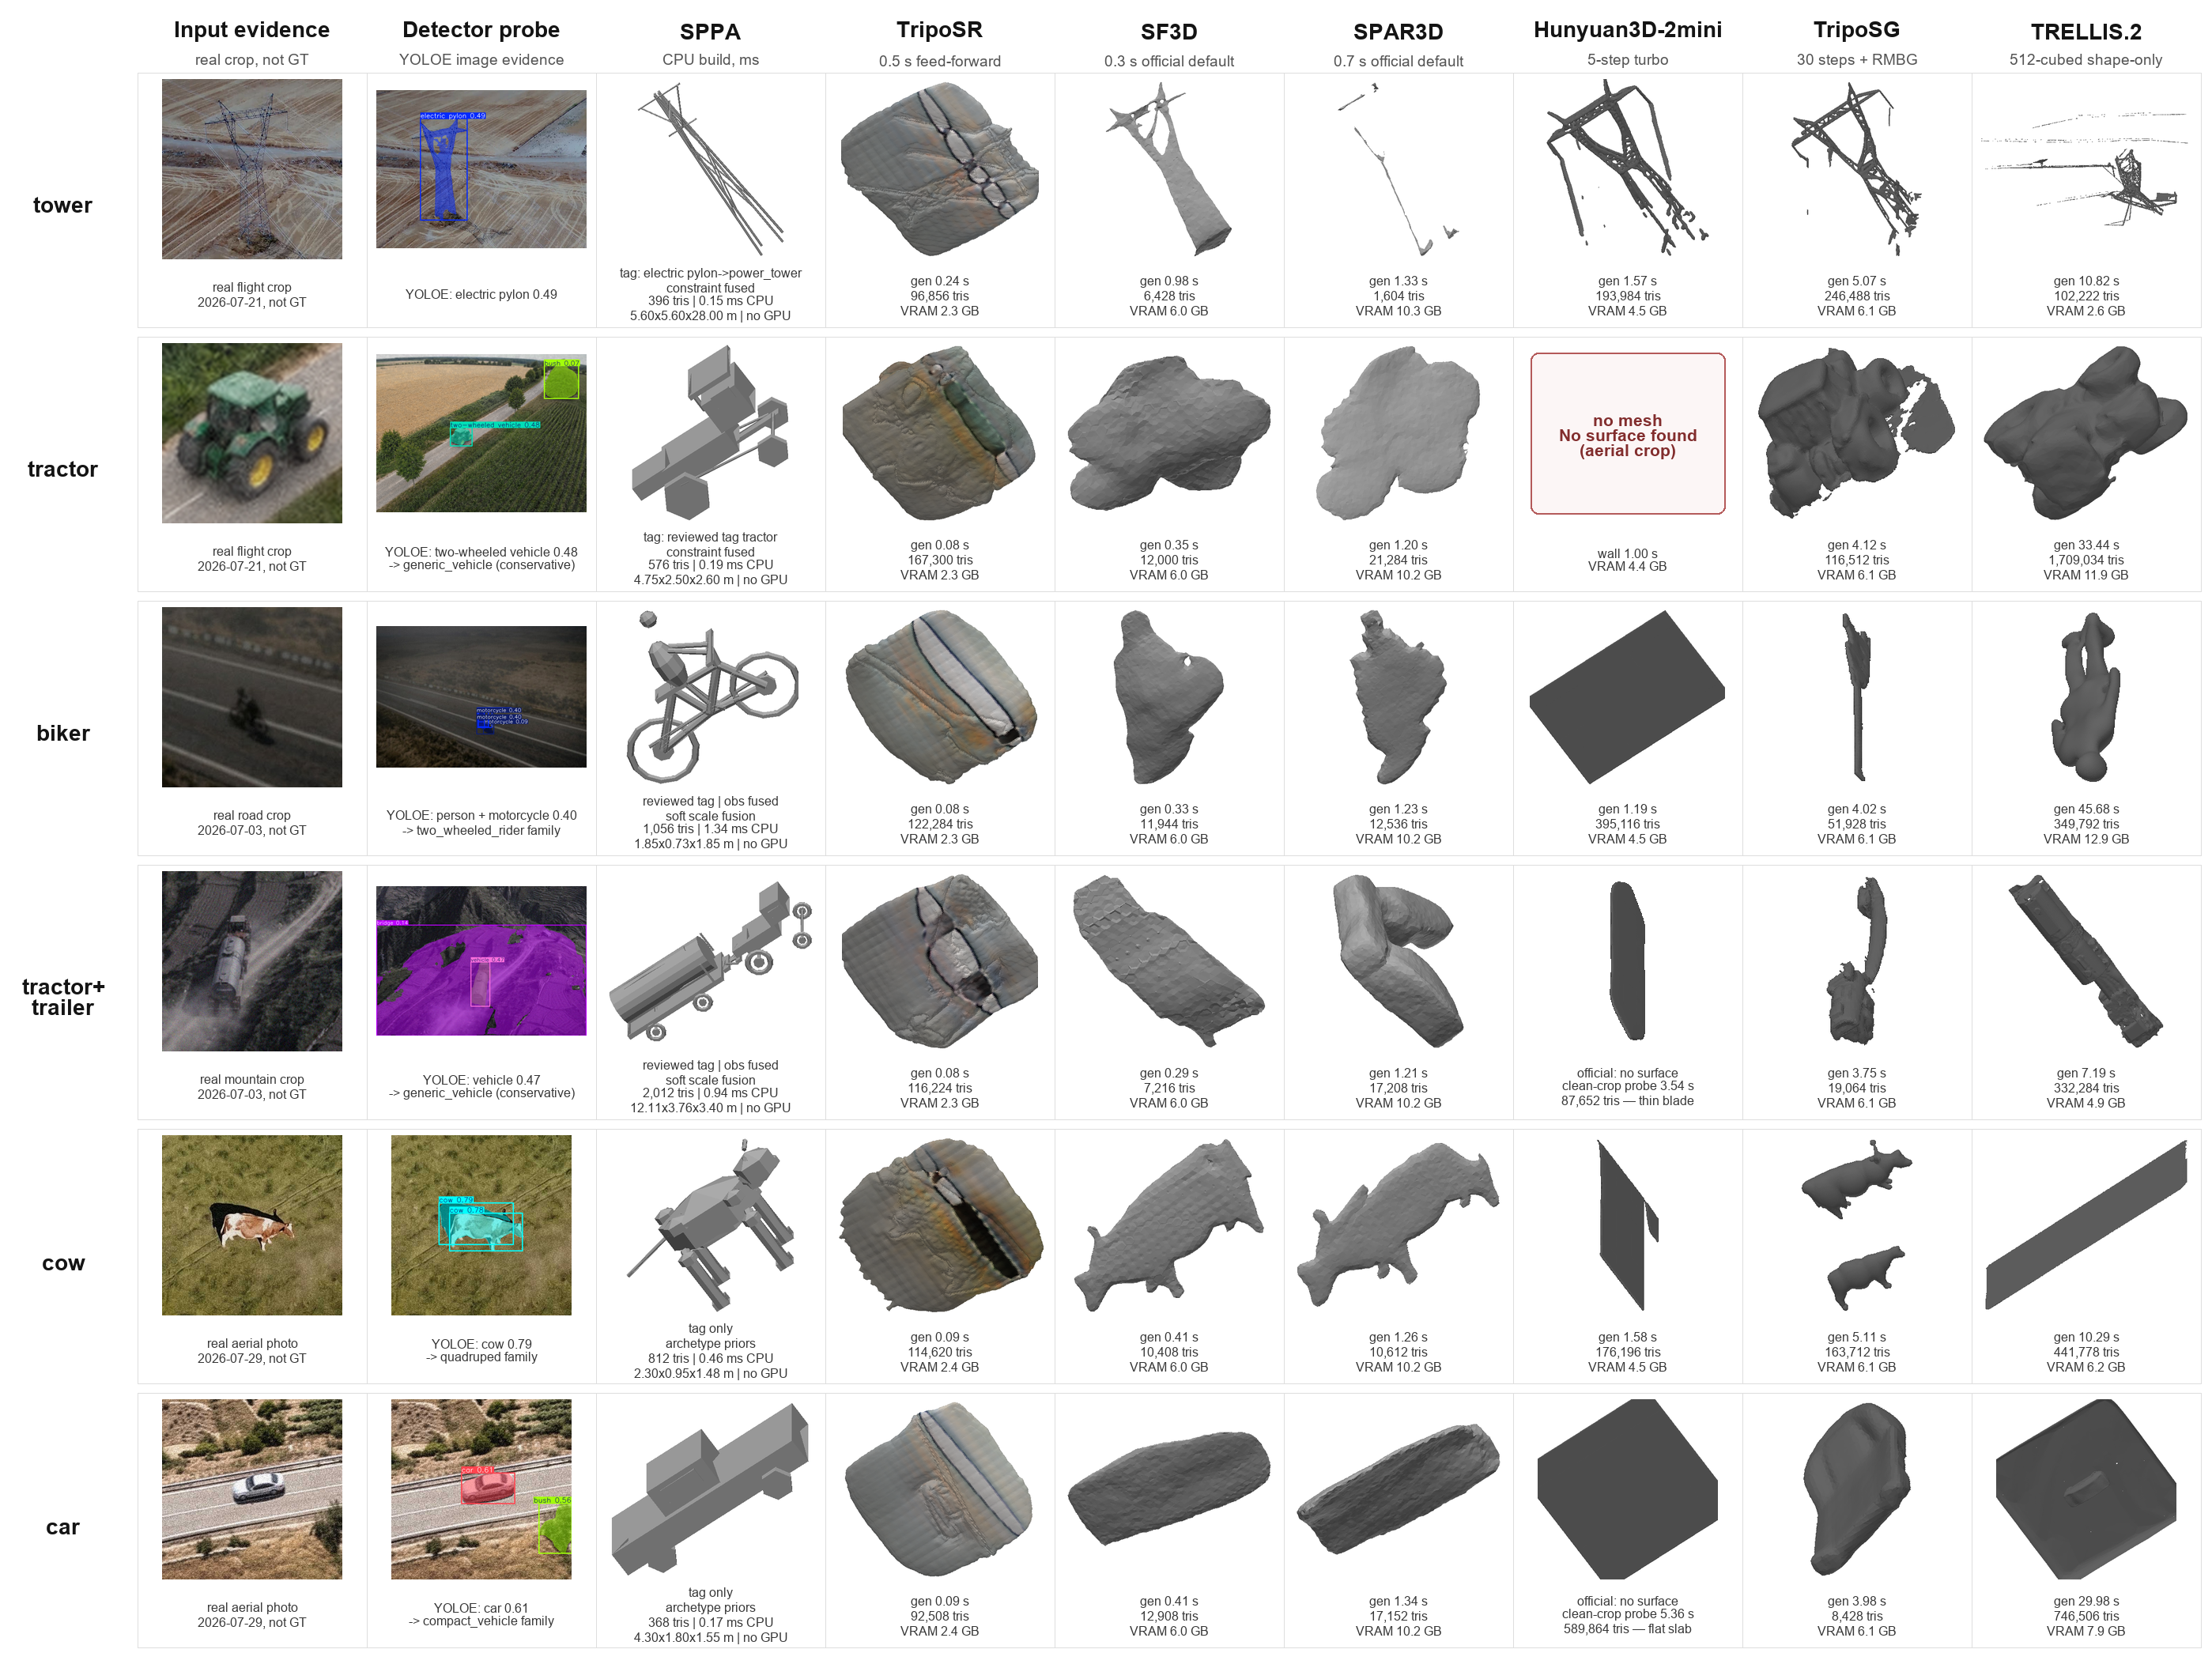
\includegraphics[width=0.95\linewidth,height=0.52\textheight,keepaspectratio]{figures/fig_hero_fastmode.png}
\caption{The operating-point argument in one view: semantic telemetry in,
displayable geometry out---SPPA against six current open 3D generators
on the same inputs, each at its fastest documented official operating point
\emph{with} its official background-removal preprocessing (exploratory; no
3D ground truth on the real crops; full per-case provenance in RP). Columns:
input crop, YOLOE-26s detector evidence, the compiled SPPA proxy (CPU,
milliseconds, no GPU), and TripoSR, SF3D, SPAR3D, Hunyuan3D-2mini, TripoSG,
and TRELLIS.2, each annotated with measured warm generation time, triangle
count, and peak VRAM on the same RTX~5090 workstation. Rows tower/tractor
are real flight crops (2026-07-21), biker/tractor+trailer real road and
mountain crops (2026-07-03), and cow/car real aerial photos (2026-07-29).
Aerial views defeat the neural columns in two distinct ways:
plausible-but-wrong geometry (blobs, flat cards) or hard failure---on the
official shared inputs Hunyuan3D-2mini returns no surface on all three
aerial vehicle crops, so its car and tractor+trailer cells show the
best-effort meshes of a debris-free manual-crop retry (same pipeline),
which exist but are degenerate (flat slab, thin blade); the tractor cell
reports the hard failure (no mesh at 5, 20, or 50 steps, on any crop).
Neural columns are qualitative context, not a ranking; measured IoU
comparisons are the sealed synthetic wave of
Section~\ref{sec:neural-external-wave}.}
\label{fig:real-flight-probes}
\end{figure}

\section{Introduction}

The motivating mission is safe remote piloting through a geospatial twin. A
pilot flies a UAV beyond visual line of sight from a portable ground
station---a laptop running a live Unreal/Cesium 3D Tiles twin, optionally
rendered through a VR headset---and must trust what the twin shows, because
a video downlink degrades with distance, weather, and interference, and at
night or in low visibility the camera ceases to be a usable primary sensor
at all. That trust breaks in a specific way: the streamed Cesium
layer is frozen at capture time, so it
shows the field as it was, not as it is now, and the operationally critical
delta---a new or relocated tower, vehicles, animals, people near the flight
path---is exactly what the static layer cannot contain. When the live image
link is degraded, the twin should absorb
whatever observation evidence does arrive and reconstruct that delta as
explicit per-object volumes, immediately and at telemetry bandwidth.

Urban and geospatial digital twins increasingly maintain live object
layers---vehicles, field equipment, temporary structures---alongside static
city geometry~\cite{batty2018digitaltwins,ogc2023tiles}, and each layer
needs a per-object 3D representation that is cheap to update in place,
explicit about uncertainty, and legible at operational zoom levels.
Semantic-telemetry UAV twins make this problem concrete: a UAV-side
perception stack reports object tracks, classes, confidence, positions, and
approximate geometry, and the ground station must render those objects in an
Unreal/Cesium 3D Tiles twin. That architectural choice creates a rendering
problem that is separate from the flight system itself: object-level telemetry
is not a mesh.

\paragraph{Scope of this paper.} We isolate exactly that rendering layer, and
we state its boundaries before the method, not after it. \emph{Localization
is assumed given}: position estimation is a separate problem solved by the
companion pipeline, whose end-to-end detector-to-twin georeferencing error
was measured at \(4\)--\(5\)~m for targets at \(40\)--\(130\)~m range, so
the actors studied here are awareness-grade volumes, not maneuvering-grade
survey. \emph{The camera is the validated sensor}: LiDAR and night, fog, or
smoke operation are evaluated only through synthetic corruptions and
simulated demonstrations, not hardware measurements. \emph{The confirmatory
domain is synthetic}: real data enters as boundary evidence and operational
case study, not as the confirmatory test. \emph{No operator benefit is
claimed}: the twin is the delivery substrate, and human-factors validation
is future work. What remains inside the claim is, we argue, the load-bearing
piece: what should be drawn, per detection, inside the twin, at what cost,
and with what measured operating envelope.

Object-level telemetry is, however, dramatically cheaper to move than the
imagery it replaces. In a recorded-flight replay of our companion telemetry
pipeline, the semantic object stream normalized to \(1.67\)~Mbps against
\(10.43\)~Mbps (H.264) and \(5.65\)~Mbps (H.265) encodings of the same
flight video---\(84.0\)\% and \(70.4\)\% lower---and the per-object update
messages measured in this paper amount to \(25.8\)--\(37.4\)~kB/s of JSON
traffic. Detection, georeferencing, and the actor lifecycle that deliver
those messages to the
twin are validated end to end in a companion manuscript; the
present paper isolates the layer that pipeline lacks: what should be drawn,
per detection, inside the twin.

Curated 3D assets are useful when the class is known, the asset library is
complete, and runtime loading is acceptable. Those assumptions are weak for
field UAV operation. Long-tail labels, ambiguous detections, partial views,
occlusion, motion blur, and changing object proportions make a fixed asset
library brittle. Neural image-to-3D and text-to-3D methods address a different
objective: visual asset generation. They produce richer geometry, but they
depend on usable crops or prompts, GPU inference, and mesh outputs too dense
for a portable flight laptop that is also running Unreal, telemetry,
video, and tracking under a shared rendering budget. The viewpoint regime
compounds the mismatch: these generators are trained and evaluated on
frontal or three-quarter studio-like views, whereas a UAV camera observes
objects from above or at grazing oblique angles, often near-nadir, where the
object must first be separated from the terrain background and most of its
3D structure is self-occluded.
Section~\ref{sec:deployment-summary} and
Figure~\ref{fig:real-flight-probes} make the mismatch concrete on real
aerial crops against six current open generators, and
Section~\ref{sec:neural-external-wave} measures the same regime
quantitatively on sealed held-out cases.

The Semantic Primitive Proxy Assembly (SPPA) takes a lower-fidelity
representation point. Instead of reconstructing
the real mesh, it compiles a detection into a semantic part graph made from
primitive boxes, cylinders, ellipsoids, cones, and tori. A vehicle becomes a
cab, body/cargo region, wheels, and optional top details. A quadruped becomes a
torso, head, and legs. A tree becomes a trunk and canopy volumes. Unknown or
unsupported labels are not hallucinated into specific objects; they fall back to
a generic uncertainty-aware display volume with explicit uncertainty metadata.
The pipeline ends in a bounded multiview silhouette fitting stage that refines
the assembled graph against calibrated top and side silhouettes; the assembly
together with this fitting stage is the single method we call SPPA throughout
(preregistered as SPPA-MVFit; protocol arms \texttt{sppa\_mvfit} for the full
pipeline and \texttt{sppa\_text\_only} for the no-fit ablation).

The question studied here is deliberately narrow and measurable. Within the
scope declared above, what the mission requires is reconstruction fidelity
under a weak signal: does a frozen semantic-family part graph improve
lightweight 3D occupancy relative to an input-matched, equal-budget
nonsemantic graph---identical silhouettes, optimizer, parameter count, and
candidate budget; only the graph changes---when both consume the same
calibrated top and side silhouettes, does the advantage survive the
corrupted observations that a weak image link implies, and can the system
itself measure when its prior should not be trusted?

The contribution is \textbf{family-conditioned SPPA}: an instant
detection-to-volume path whose semantic prior is validated by a
preregistered, equal-budget comparison showing that the family graph
improves clean voxel IoU over a generic eight-part graph by \(0.190\) (95\%
CI \([0.181,0.199]\)) on 240 held-out synthetic actors, together with a
measured operating envelope that maps where the prior helps, where it hurts,
and where it stops transferring. The optimizer is deliberately a shared
five-parameter global alignment and is not claimed as a novel fitting
algorithm.
Concretely, the paper contributes: (i)~an instant detection-to-volume
path---a reviewed family recipe compiles one detection into a role-labeled
eight-part actor in \(9.4\)~ms median CPU per object, emitted as a compact
\(1.45\)~kB update descriptor, and sustains \(11.8\)~ms median per detection
on a real 2--15~Hz detector stream; (ii)~preregistered evidence of volumetric
fidelity and of robustness to a weak signal---the advantage
is maintained under all prespecified mask and morphology
corruptions, and the frontier where it stops is measured (wrong-family
tokens, adversarial family instances, external real meshes, and a real
detector stream); (iii)~the twin-delta update contract---role labels,
bounded in-place updates, telemetry-scale JSON update traffic, and an
operational part-query
value (F1 \(0.434\))---with its declared limits; and (iv)~a measured
trust-gating policy for the contract itself: on the real stream, detector
confidence plus prior fit separate wrong from correct family tokens (AUC
\(0.847\), 95\% CI \([0.792,0.898]\)), and a frozen routing rule lifts
stream-level median 2D IoU from \(0.298\) to \(0.432\) by committing only
the \(19\%\) most confident detections to family proxies---the operating
pattern we argue every family-conditioned twin layer needs.

\section{Related Work}

\paragraph{Geospatial digital twins and dynamic object layers.}
Semantic 3D city models provide the static substrate: CityGML and CityJSON
structure city objects with semantics and levels of
detail~\cite{ledoux2019cityjson,biljecki2015applications}, and digital-twin
reviews identify live, sensor-fed object layers---not the static model---as
the open technical gap~\cite{ketzler2020digitaltwins,batty2018digitaltwins}.
For moving or temporary objects, geovisual analytics of movement analyzes
trajectories and events~\cite{andrienko2013movement}, but the per-object
volumetric primitive a 3D twin should \emph{draw} from sparse detections is
largely unspecified. A parallel GIScience literature establishes that
uncertainty in spatial displays must be designed, not
improvised~\cite{maceachren2005visualizing}; SPPA adopts this as contract
requirements---every actor carries role-labeled uncertainty metadata, an
explicit \texttt{yaw\_ambiguous} flag, and a conservative fallback volume
rather than a hallucinated object. Finally, UAV photogrammetry quantifies
the observation regime behind our error modes: nadir and oblique airborne
views constrain footprint geometry well but recover height poorly from
monocular evidence~\cite{nex2014uav}---exactly the evidence-versus-prior
tension the real stream of Section~\ref{sec:real-stream} measures. SPPA is,
to our knowledge, the first attempt to give the dynamic object layer of a
UAV geospatial twin an explicit, bounded, telemetry-driven volumetric
contract.

Text-to-3D and image-to-3D generators target visual asset fidelity from prompts
or images
\cite{poole2022dreamfusion,lin2022magic3d,nichol2022pointe,tochilkin2024triposr,sf3d2024,stability2025spar3d,triposg2025,xu2024instantmesh,xiang2024trellis,xiang2025trellis2,zhao2025hunyuan3d}.
SPPA targets a different runtime point: deterministic actor generation from
sparse semantic telemetry, low polygon counts, and cheap per-frame updates.

Monocular and open-vocabulary 3D detection estimate 3D boxes or object state
from images \cite{brazil2022omni3d,yao2024ovmono3d}; YOLOE supplies approximate
open-prompt detection/segmentation evidence rather than universal recognition
\cite{wang2025yoloe}. Animal pose and
reconstruction methods estimate detailed skeletons or category-specific 3D
shape \cite{yu2021ap10k,li20243dfauna,hu2026sam3danimal}. These methods can
provide stronger evidence to SPPA, but SPPA itself is a rendering/backend layer,
not a detector or pose estimator.

Category-conditioned parametric templates are the closest established paradigm.
3D morphable models fit a low-dimensional learned face prior to image
evidence~\cite{blanz1999morphable}, and articulated body and animal models such
as SMPL and SMAL fit a category-conditioned parametric template to scans or
images~\cite{loper2015smpl,zuffi2017smal}. SPPA instantiates the same
pattern---a family-conditioned template aligned to observation evidence---with
an eight-part primitive graph and a deliberately shared five-parameter global
alignment. The operating point differs: SPPA targets millisecond,
track-updateable display actors from sparse UAV telemetry rather than
surface recovery of a specific category.

{\sloppy
Primitive representations have a long history, from volumetric primitives,
recognition-by-components, and superquadrics to learned part decomposition and
neural primitive/CSG parsing
\cite{biederman1987recognition,solina1990recovery,paschalidou2019superquadrics,tulsiani2017learning,mo2019partnet,sharma2018csgnet,fedele2025superdec}.
Procedural modeling, shape grammars, and learned shape programs generate or
abstract structured objects from compact programs
\cite{mueller2006procedural,jones2020shapeassembly,jones2023shapecoder,khan2024text2cad,rukhovich2024cadrecode}.
\par}
SPPA uses these ideas operationally, but the claimed novelty is the bounded,
track-updateable semantic telemetry contract inside an Unreal UAV digital twin.

Recent scene-level systems narrow the gap from other directions: SAM 3D
decomposes a single image into composable per-object geometry
\cite{chen2026sam3d}, PartCrafter generates part-structured meshes from one
image \cite{lin2025partcrafter}, SuperQuadricOcc reaches real-time semantic
occupancy in driving scenes \cite{hayes2025superquadricocc}, and lightweight
urban twins render proxy building geometry at interactive rates
\cite{liu2025citygo}; we are not aware of any that constructs role-labeled,
metric-scaled object actors from detector tags and sparse silhouettes at
millisecond cost.

Graphics systems already provide level-of-detail, impostors, billboards,
streaming tiles, and virtualized geometry \cite{clark1976hierarchical,decoret2003billboard,epic2026nanite,ogc2023tiles}.
3D and dynamic scene graphs maintain semantic world structure
\cite{armeni2019scenegraph,rosinol2020dynamic,wu2021scenegraphfusion}, and
Hydra-style systems build hierarchical scene graphs online for mapping and
planning \cite{hughes2022hydra}; SPPA deliberately keeps its own lightweight
display-actor contract---a bounded descriptor/update payload---instead of
becoming a node type in such a substrate, and it should be read as a display
actor that can consume upstream occupancy evidence (OctoMap, ESDF, TSDF
\cite{hornung2013octomap,oleynikova2017voxblox}), not as a mapping layer.

Table~\ref{tab:sota-positioning} positions SPPA against these paradigms
on the properties that matter for a telemetry-driven UAV twin. To our
knowledge, no current paradigm simultaneously
(i)~consumes detector-level telemetry rather than pixels or prompts,
(ii)~emits a role-labeled low-polygon actor rather than a dense mesh or a
category surface, (iii)~updates that actor in place at millisecond CPU cost,
and (iv)~exposes a bounded descriptor/update contract to the renderer; each
row of the table fails at least one of the four. SPPA is designed for
exactly this conjunction.

\begin{table}[!htb]
\centering
\scriptsize
\setlength{\tabcolsep}{3pt}
\caption{Positioning of SPPA against state-of-the-art paradigms for
per-object 3D in a telemetry-driven UAV digital twin. \emph{Telemetry input}:
consumes detector tags/footprints rather than RGB or prompts. \emph{Role
labels}: named semantic parts, not anonymous geometry. \emph{In-place update}:
pose/shape updates without regenerating the actor. Cost is the per-object
generation cost at the cited systems' operating points.}
\label{tab:sota-positioning}
\begin{tabularx}{\linewidth}{@{}L{0.235\linewidth}Y Y Y Y@{}}
\toprule
Paradigm (representative systems) & Telemetry input & Role labels & In-place update & Per-object cost \\
\midrule
Neural image/text-to-3D (TripoSR, SF3D, SPAR3D, Hunyuan3D-2, TripoSG, TRELLIS.2) & no (image/prompt) & no & no & 0.08--46~s GPU; 1.6k--3.4M tris; 2--16~GB VRAM \\
Category templates (3DMM, SMPL, SMAL) & no (scans/images) & category-specific & partial & offline fitting \\
Learned primitive decomposition (SuperDec, DualPrim, superfrusta) & no (image/cloud) & implicit parts & no & GPU inference \\
Scene graphs (Hydra, 3D DSG) & mapping sensors & object level & yes & mapping layer, not a display actor \\
LOD / impostors / billboards & no (needs assets) & no & yes & negligible, but asset required \\
Occupancy maps (OctoMap, voxblox) & depth sensors & no & yes & navigation map, not actors \\
\bottomrule
\end{tabularx}
\end{table}

\section{Materials and Methods}

\subsection{The SPPA pipeline end to end}
\label{sec:architecture}

The SPPA path compiles one incoming detection into a live actor in the twin
through six deterministic stages. The whole
path is rule-based and reviewed---no neural network runs anywhere in it, and
no geometry is ever invented at runtime.

\paragraph{Stage (1) --- Telemetry input.}
At time \(t\), SPPA consumes an object state
\[
x_t = \{i, \ell, c, b_t, m_t, \xi_t, s_t, \Sigma_t, h_t\},
\]
where \(i\) is a track identifier, \(\ell\) a detector label, \(c\) confidence,
\(b_t\) a bounding region, \(m_t\) an optional mask or footprint, \(\xi_t\) a
world pose estimate, \(s_t\) optional metric dimensions, \(\Sigma_t\)
uncertainty, and \(h_t\) the track history.

\paragraph{Stage (2) --- Resolve label: reviewed recipes, no runtime invention.}
The resolver maps \(\ell\) to one of
three cases: an \texttt{exact\_class} label with a fixed archetype; a
\texttt{keyword\_archetype} mapping of an out-of-template label to a finite
reviewed archetype, such as vehicle or vertical structure; or a
\texttt{fallback\_unknown\_label} rendered as a generic uncertainty-aware
volume. The versioned recipe manifest covers 23 archetypes and 95 exact or
keyword labels; SPPA can accept an open detector tag at runtime, but the tag is
normalized into a reviewed family or a conservative unknown fallback before
geometry is emitted. An adversarial resolver audit over 12 compound or
misleading labels is included
in RP (\texttt{reproducibility/sppa\_mvfit/};
\emph{RP} below).

Who writes the recipes is part of the contract. Candidate part
decompositions may be drafted offline by a language model, an ontology tool,
or a human author, but a draft is admitted only after human review,
regression tests, and versioned freezing; no language model runs at runtime.
The count, primitive types, roles,
and slot arrangement of every emitted actor therefore come from a frozen
recipe: the system can scale, clamp, fit, or fall back, but it cannot
hallucinate an unreviewed part topology.

Coverage is explicit, not implied. The open-vocabulary detector
(YOLOE-26s) runs an operator-frozen prompt list at launch (52 class prompts
in the universal profile, 9 in the flight profile), and the ontology routes
64 exact labels and 92 keyword mappings into the reviewed families
(\texttt{SPPA-ONTOLOGY-0.4}); anything outside both becomes the fallback
uncertainty volume by design, never a hallucinated object. Family routing
gives open-set coverage without recipe proliferation, measurably: a
\emph{giraffe}---no recipe anywhere in the manifest---is detected zero-shot
(confidence \(0.918\) on an external ground-level photo) and compiled
through the reviewed \texttt{quadruped} family into a role-labeled proxy at
evidence dimensions (\(3.80\times1.50\times4.80\)~m, 580 triangles), with no
giraffe-specific recipe ever frozen; what the family cannot express (the
neck proportions) is the part-structure limit declared in
Section~\ref{sec:threats}.

\paragraph{Stage (3) --- Evidence gate: Observe, Project, Scale, Gate.}
\label{sec:pipeline}
Both input contracts terminate in the same deterministic builder; they differ
only in how much evidence reaches the recipe. The tag/text path compiles a
reviewed recipe at its prior dimensions: normalize the label through the
reviewed ontology, select the frozen part graph \(G_a\) and its prior role
parameters, and emit the versioned descriptor consumed once
per track by the renderer. The detector/image path inserts four evidence
stages before the same builder: (1)~\textbf{Observe}---detector label,
confidence, bbox, and native mask polygon are stored in a
\texttt{SPPA-OBS-0.1} record with declared camera/flight geometry and an
uncertainty envelope; (2)~\textbf{Project}---the mask polygon
is projected through the declared camera model into an oriented ground
footprint; (3)~\textbf{Scale}---with declared metric calibration the
footprint becomes a metric length/width/height proposal; without calibration
the mask remains image-space evidence and cannot change metric geometry;
(4)~\textbf{Gate}---a class-aware constraint-fusion step accepts plausible
scale, clamps implausible length/width ratios through the family aspect prior,
withholds unsafe image-derived pose/yaw from the runtime descriptor, and
records every decision with its reason. Because both paths share the builder
and the descriptor contract, their outputs are directly comparable.

The evidence contract is sensor-agnostic by design: any sensor that
delivers an oriented ground footprint geo-projected from its observation,
with declared geometry and uncertainty, enters the same gate and the same
builder. The camera path is the validated one---exercised by the real-image
probes of Section~\ref{sec:deployment-summary} and by the recorded detector
stream of Section~\ref{sec:real-stream}; LiDAR reduces to the same
geo-projected footprint by design, but no hardware LiDAR measurement is
reported here---the camera-less
path is exercised only in a simulated-LiDAR twin demonstration retained in
RP, and night, fog, or
smoke operation is likewise evaluated only through
the prespecified synthetic mask corruptions of
Section~\ref{sec:robustness}, not through measured degraded-weather data.

\paragraph{Worked example (tractor-trailer probe).}
The real crop yields YOLOE evidence \texttt{vehicle} at confidence 0.47 with a
54-point native mask. Projection proposes a raw footprint of
\(16.85\times6.21\times3.40\) m; the gate applies soft low-confidence fusion,
clamps the footprint through the vehicle aspect prior to
\(12.11\times3.76\times3.40\) m, withholds image-derived pose, and refines the
weak label only to the conservative \texttt{articulated\_vehicle} family. The
shared builder then emits a 1{,}904-triangle proxy (evidence in RP).
The full chain is written out step by step in RP, including a measured
detection of the real stream of Section~\ref{sec:real-stream} traced through
every stage.

\paragraph{Stage (4) --- Build proxy: the frozen family part graph.}
Each archetype \(a\) defines a part graph
\[
G_a = (V_a,E_a), \quad v_k = (p_k,r_k,\tau_k,\rho_k),
\]
where \(p_k\) is a primitive type, \(r_k\) is its role, \(\tau_k\) its transform
relative to the actor root, and \(\rho_k\) role-specific parameters such as
dimension priors, color/material role, and confidence tags. The current
implementation uses boxes, cylinders, ellipsoids, cones, and tori
(Figure~\ref{fig:family-graphs}).

\begin{figure}[!htb]
\centering
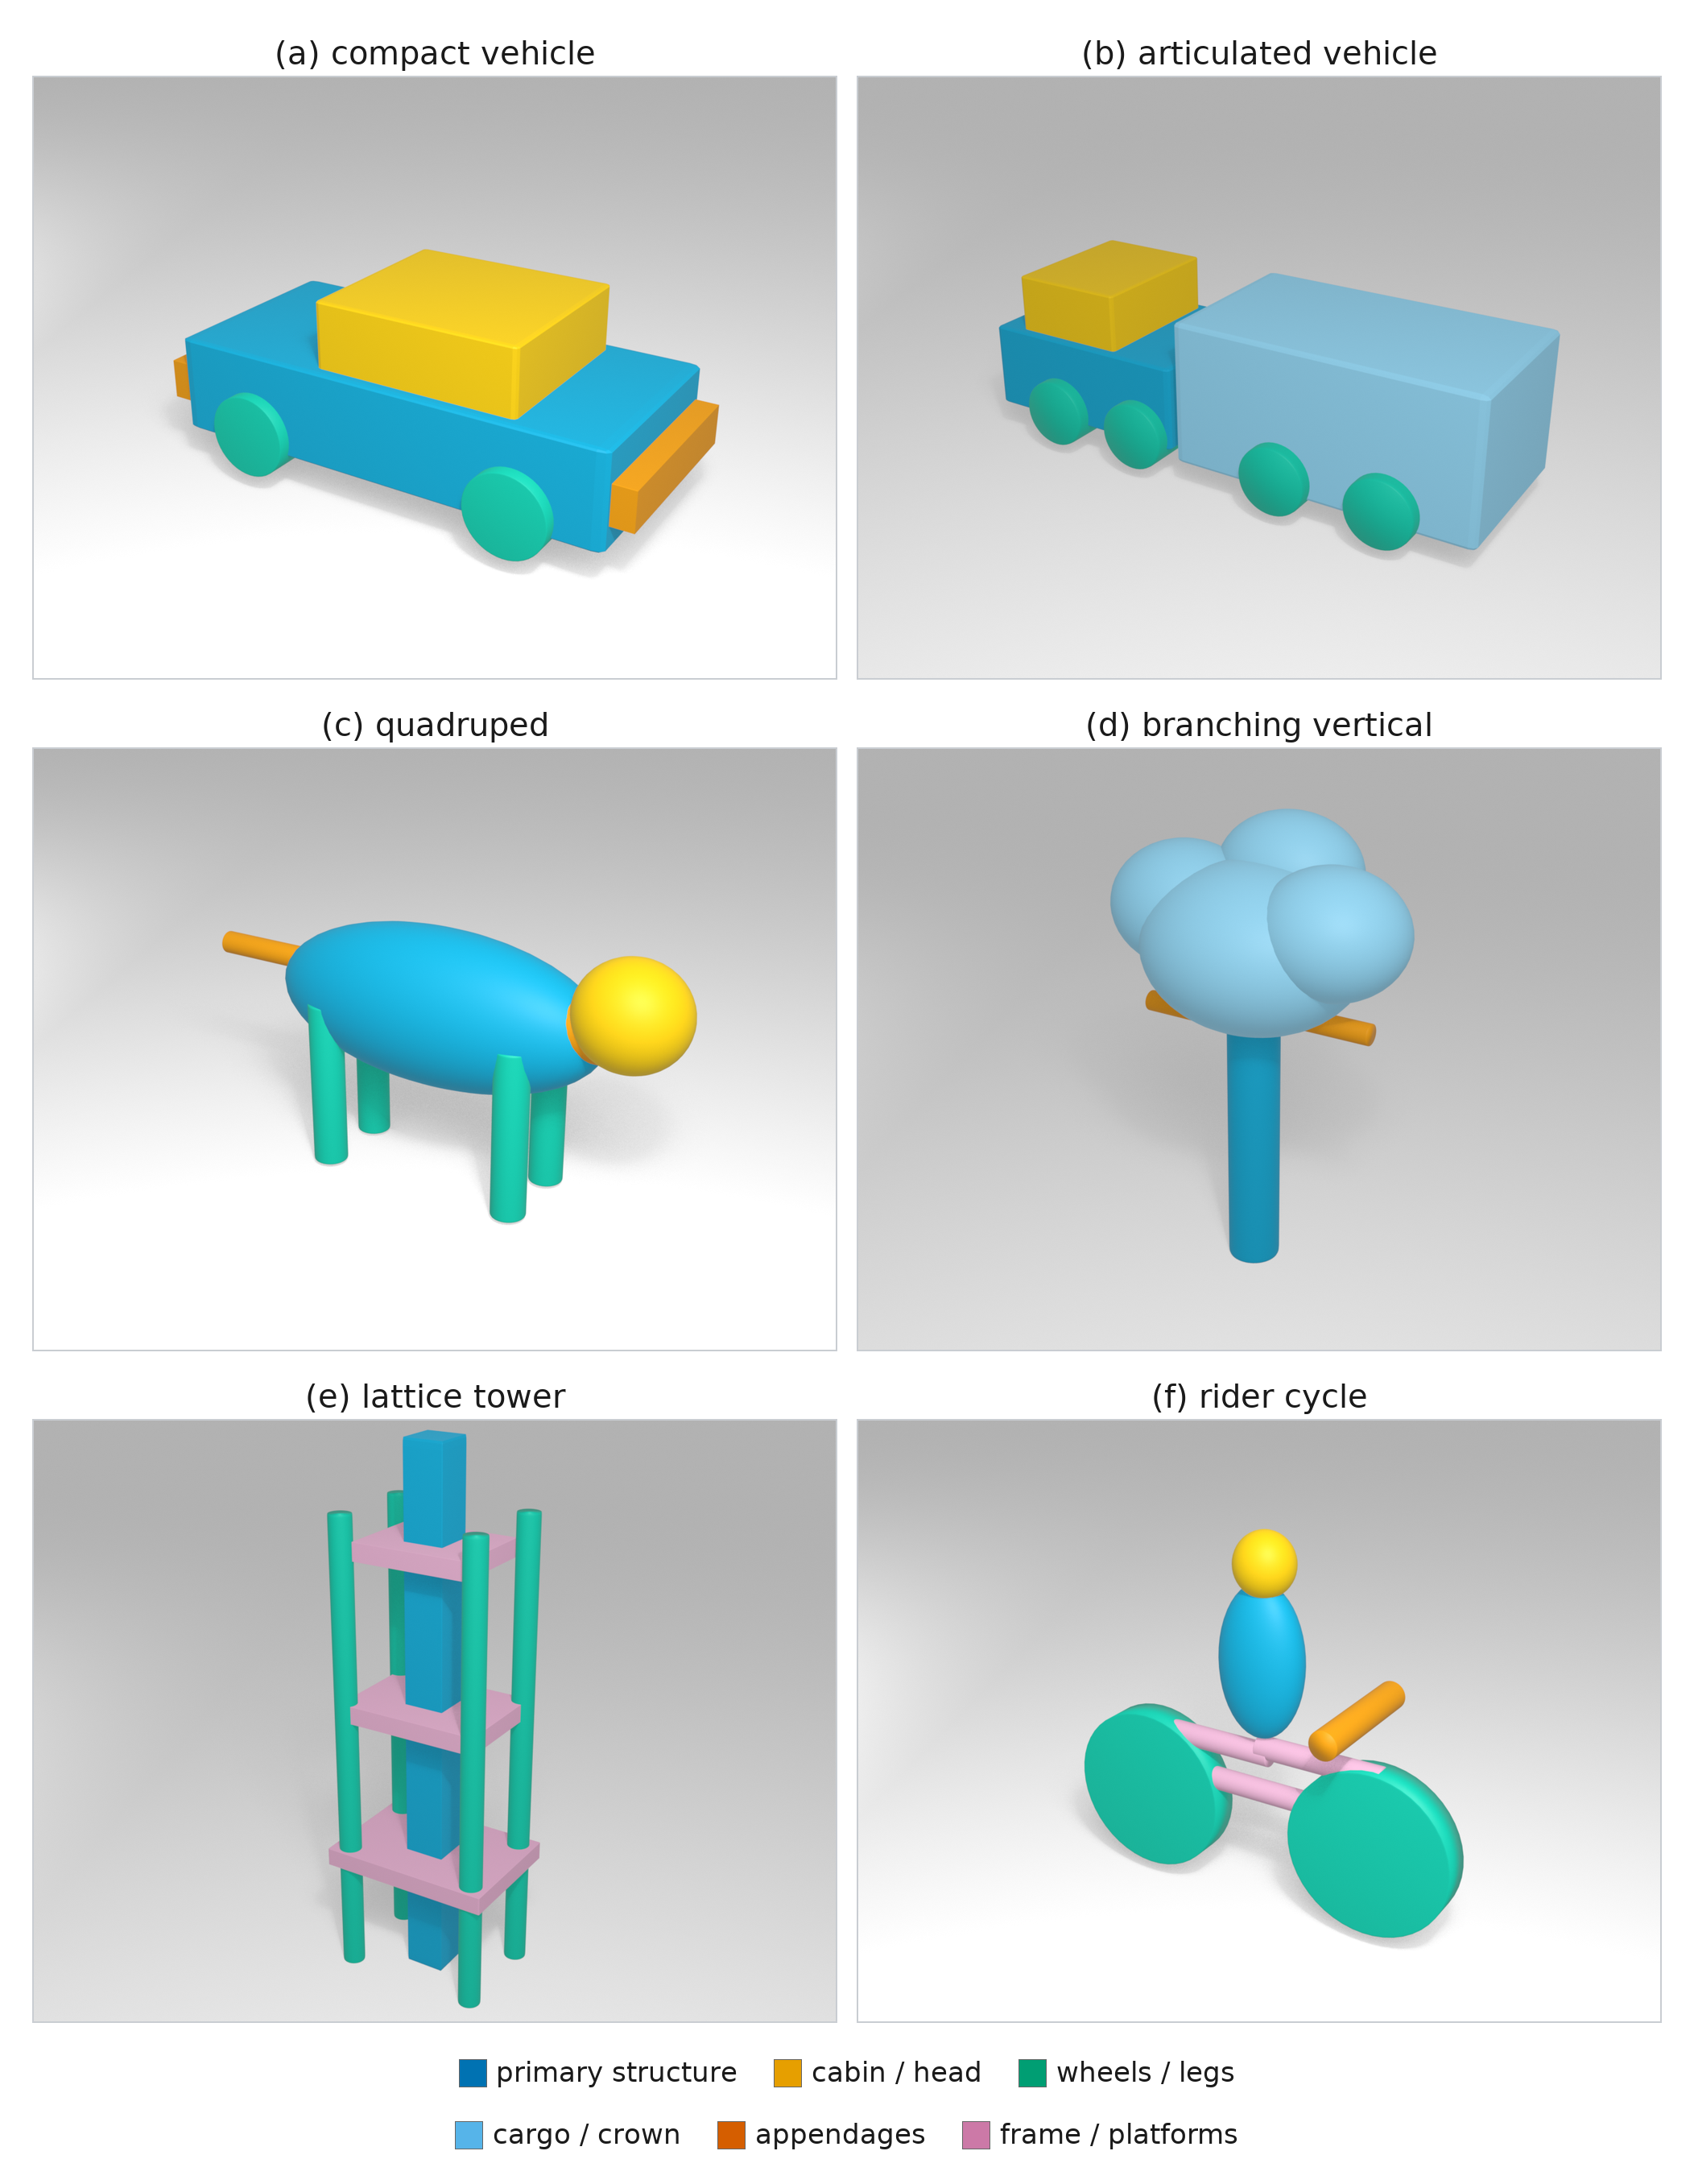
\includegraphics[width=0.6\linewidth,height=0.32\textheight,keepaspectratio]{figures/fig_family_graphs_blender.png}
\caption{The six benchmark family part graphs used by SPPA
(\texttt{compact\_vehicle}, \texttt{articulated\_vehicle}, \texttt{quadruped},
\texttt{branching\_vertical}, \texttt{lattice\_tower}, \texttt{rider\_cycle}):
eight primitive slots per family with role-conditioned priors; colors denote
semantic roles.}
\label{fig:family-graphs}
\end{figure}

Part placement is a recipe prior, not a runtime decision: the slot
transforms \(\tau_k\) and role priors \(\rho_k\) position every part, and
runtime stages may scale or clamp them but never reposition individual
parts. In the production \texttt{quadruped} recipe, for example, which
primitive, in which
count, carrying which role is \emph{knowledge}---authored offline, reviewed,
regression-tested, and frozen in the recipe; each part's instance position
and scale is \emph{computation}---derived in real time from the
evidence-driven dimensions through role coefficients clamped to declared
ranges (the full anatomy table is in RP). The count is the smallest set that
covers the family's occupancy modes---alternative decompositions were
measured and rejected (Section~\ref{sec:generic-sensitivity}).

Vehicle adaptation is the clearest implemented case: in the current
vehicle grammar, cab and wheel dimensions remain bounded by role priors,
while the cargo/body span and axle placement absorb length changes, so a
long truck and a short truck are not produced by globally scaling the same
box (synthetic truck check in RP).

\paragraph{Stage (5) --- Optional fit: one global five-parameter alignment.}
When calibrated top and side silhouettes are available, SPPA refines
the assembled graph with a single shared parameter vector
\(\theta=(\log s_x,\log s_y,\log s_z,s_{\mathrm{sec}},o_{\mathrm{sec}})\)
applied to all eight slots at once, optimizing silhouette agreement over a
fixed 31-candidate budget (the exact loop is
Algorithm~1 of Section~\ref{sec:mvfit}). The fit is deliberately global: it
scales and spans the assembled family graph as one object and never moves
parts independently. That restriction keeps the path deterministic,
millisecond-cheap, and contract-stable, and its cost is measurable:
structures that violate the family prior degrade in identifiable zones
(Section~\ref{sec:adversarial}).

\paragraph{Stage (6) --- Twin update: descriptor, pose, and lifecycle.}
\label{sec:implementation}
{\sloppy
A \texttt{SPPA-DESC-0.2} record carries the resolved family, the role-labeled
part list, and the evidence, uncertainty, and material tags needed to build
the actor once per track; a \texttt{SPPA-UPD-0.2} record separates
create/regenerate payloads from the pose/no-op/shape updates applied in place
(field-level contents and the \texttt{descriptor\_id}
topology-cache identity rule in RP). The
design goal is to generate once per track/archetype, update
pose/material/uncertainty every frame, and apply shape-parameter changes in
place when the part topology is unchanged. An optional Unreal Engine 5.7
backend ingests the same descriptors alongside curated assets, which remain
the default, and rejects invalid JSON or mismatched descriptor identifiers
without changing the current actor.
\par}
The descriptor separates actor pose \(\xi_t\) from part parameters \(q_t\). Yaw
ambiguity is handled explicitly: a top-down footprint or PCA orientation gives
an axial orientation modulo \(\pi\), and signed yaw requires velocity,
asymmetry, multi-frame evidence, or an external heading source; otherwise the
descriptor sets \texttt{yaw\_ambiguous=true}.

\subsection{Confirmatory protocol}
\label{sec:mvfit}

Every compared method receives the same case identifier, morphology-family
token, metric world box, and two \(96\times 96\) orthographic binary
silhouettes (top and side). No method receives RGB pixels, detector scores,
source parameters, ground-truth occupancy, evaluation projections, or real or
replay telemetry. An actor is an ordered list of eight primitive slots (boxes,
cylinders, ellipsoids). Family graphs and a single \texttt{generic} graph are
stored as static JSON. The only builder used by the text-only ablation, the
Generic graph baseline, and SPPA is
\begin{equation}
A = \mathrm{Build}(g,\theta),\qquad
\theta=(\log s_x,\log s_y,\log s_z,s_{\mathrm{sec}},o_{\mathrm{sec}}),
\end{equation}
with identical bounds for every graph \(g\). The text-only ablation (SPPA
without the fitting stage; protocol arm \texttt{sppa\_text\_only}) uses the family
graph at the default \(\theta_0\); the Generic graph baseline and SPPA optimize the
same five parameters under the same objective and candidate budget, and only
the graph identity differs (\texttt{generic} vs family). The fitting loop is
written out exactly in Figure~\ref{alg:mvfit}. Baselines include
axis-aligned box, ellipsoid, capsule, billboard, and nonsemantic visual hull
from the same masks.

\begin{figure}[!htb]
\centering
\fbox{\begin{minipage}{0.88\linewidth}
\footnotesize
\textbf{Algorithm 1 --- SPPA: 31-candidate silhouette fit
(identical for every compared graph \(g\)).}\\[3pt]
\textbf{Input:} graph \(g\); binary silhouettes \(S_{\mathrm{top}}\),
\(S_{\mathrm{side}}\) (\(96{\times}96\)); metric world box.\\
\textbf{Parameters:} \(\theta=(\log s_x,\log s_y,\log s_z,s_{\mathrm{sec}},
o_{\mathrm{sec}})\), shared by all eight slots.\\
\textbf{Objective:} \(J(\theta)=0.5\,(1-\mathrm{IoU}_{\mathrm{top}})
+0.5\,(1-\mathrm{IoU}_{\mathrm{side}})+\varepsilon\cdot\)centering,
evaluated on the actor's projections against the observed silhouettes.\\[2pt]
\begin{enumerate}[leftmargin=1.6em,itemsep=0pt,topsep=1pt]
\item Initialize \(\theta_0\) from the observed mask extents; evaluate
\(J(\theta_0)\) \hfill(1 evaluation)
\item For each step fraction \(f\in\{0.10,\,0.03,\,0.01\}\) (three shrinking
sweeps): for each of the five parameters, evaluate \(J\) at the current best
\(\theta\) with that parameter moved by \(\pm f\) times its allowed range, and
keep the better value \hfill(\(3\times5\times2=30\) evaluations)
\item Return \(\theta^{\ast}\). Total cost: exactly \(1+30=31\) objective
evaluations for every method---the budget is part of the controlled
comparison, not a tuned choice.
\end{enumerate}
\end{minipage}}
\caption{The complete fitting loop used by SPPA and Generic graph. The
only difference between the two methods is the graph \(g\) passed to the
shared builder; the parameterization, bounds, objective, initialization, and
candidate budget are identical.}
\label{alg:mvfit}
\end{figure} The fitter is deliberately a five-parameter global
alignment shared by all slots; the contribution is the family-conditioned
representation and the runtime contract, not the optimizer (a fitted example
sequence is included in RP).

The \texttt{generic} graph was designed by the authors as a plausible
family-agnostic prior: eight symmetric ellipsoid slots with no
family-specific topology, proportions, or role labels, frozen before the
benchmark was run. It is hand-crafted, not learned, not random, and not the
mean of the six family graphs. Because the same team authored the family
graphs and this generic competitor, three alternative generic graphs were
registered in writing before any measurement and are evaluated in
Section~\ref{sec:generic-sensitivity}; the shared-authorship threat is
discussed in Section~\ref{sec:threats}.

The primary hypothesis compares clean-mask 64-cubed voxel IoU of SPPA
against Generic graph. Analysis units are 240 source actors (20 per family in
each of two strata). The confirmatory estimand is the equal-stratum mean paired
difference. H1 passes only if the lower endpoint of a two-sided 95\% stratified
actor-bootstrap percentile interval (10{,}000 resamples, seed 77157) exceeds
\(+0.030\). The margin and the power analysis behind the sample size were fixed
before evaluation: with paired-difference SD \(0.12\), \(n{=}240\) actors give
approximately 90\% normal-approximation power to distinguish a true mean of
\(+0.055\) from the \(+0.030\) margin. The full protocol was preregistered
and sealed before evaluation; the seed provenance, amendment log, and freeze
records are given in RP. Two amendments to the sealed
protocol are disclosed: Amendment~03 substituted the planned external review
of the protocol (not obtainable) by an internal triple-role self-audit, and
Amendment~04 re-derived the secondary inference after the seal (null-centered
bootstrap with Holm adjustment). Development results
were used only to implement the frozen package and are not confirmatory.

Source actors come from two strata: CSG-ID unions of solids with family
topology, and implicit-OOD occupancy from superelliptic extrusions,
taper/twist, toroidal sections, and spline-distance tubes. Source and method
modules do not import each other. The held-out set is developer-held-out
synthetic geometry, not an externally blinded public UAV benchmark.

All confirmatory and post-hoc fits ran on one benchmark workstation (AMD
Zen~5, 32 logical CPUs, Windows~11, CPython 3.12.6); the external
neural-generator runs of Section~\ref{sec:neural-external-wave} used an
RTX~5090 32~GB GPU on the same machine. We state the hardware context
explicitly because the motivating mission is a portable flight laptop:
``instant'' throughout this paper is a per-object CPU wall-clock claim at
this workstation class, not a measured flight-laptop frame time, and
dense-scene rendering limits are reported separately in
Section~\ref{sec:deployment-summary}.

\subsection{Evaluation data}
\label{sec:evaluation-data}

The synthetic benchmark covers six families selected before freezing for
morphological coverage of the ground-object envelope a UAV twin must display:
compact rigid bodies (\texttt{compact\_vehicle}), elongated articulated bodies
(\texttt{articulated\_vehicle}), legged organic forms (\texttt{quadruped}),
branching vertical growth (\texttt{branching\_vertical}), thin lattice
structures (\texttt{lattice\_tower}), and rider-plus-cycle combinations
(\texttt{rider\_cycle}). A post-hoc exploratory drop-one-family re-analysis
(Section~\ref{sec:results-decomposition}) confirms the headline difference is
not carried by any single family: excluding any one family leaves the paired
difference between \(0.152\) and \(0.214\), always above the \(+0.030\)
margin. As an external case study outside the design distribution, the same
methods were run on \(n{=}52\) real third-party meshes (Objaverse LVIS subset
and ModelNet40) under a class-to-family mapping frozen in writing before any
evaluation (Section~\ref{sec:external-sanity}). Real-image probes (four
archived field crops and two real flight photos of a tower and a tractor
recorded for
this paper on 2026-07-21) exercise the dual-input contract of
Section~\ref{sec:pipeline} with a
YOLOE-26s open-vocabulary detector (checkpoint \texttt{yoloe-26s-seg.pt}) as
approximate semantic evidence (Section~\ref{sec:deployment-summary}).

\section{Results}
\label{sec:primary-results}

\subsection{Primary confirmatory result}

Table~\ref{tab:mvfit-h1} reports the confirmatory decision: H1 passes, with
mean \(\Delta\mathrm{IoU}=0.190\) and 95\% CI \([0.181,0.199]\). The CSG-ID
stratum mean difference is \(0.209\) and the implicit-OOD stratum mean
difference is \(0.172\); neither is non-positive, so a cross-stratum
generalization warning is not triggered by the protocol rule. The OOD
stratum---built by a generator that does not instantiate the CSG family
topology---is also the in-benchmark guard against a design-decided result,
and the margin persists there. The
structural-favor threat itself is bounded by measurement in
Sections~\ref{sec:adversarial} and~\ref{sec:generic-sensitivity} and
discussed in Section~\ref{sec:threats}.
Figure~\ref{fig:h1-by-family} and Table~\ref{tab:family-stratum} report the
paired difference in every family-by-stratum cell. All twelve point estimates
are sealed and positive: the largest gain is \texttt{rider\_cycle} CSG-ID
(\(+0.458\), CI \([0.402,0.508]\)) and the smallest is
\texttt{compact\_vehicle} implicit-OOD (\(+0.043\), CI \([0.028,0.057]\)),
and the drop-one-family re-analysis of Section~\ref{sec:evaluation-data}
confirms that no single family carries the headline.

\begin{table}[!htb]
\centering
\footnotesize
\caption{Preregistered primary endpoint on the held-out synthetic test
(\(n{=}240\) actors). Provenance: \texttt{synthetic\_geometry}. H1 passes only
if the stratified bootstrap 95\% lower bound exceeds \(+0.030\).}
\label{tab:mvfit-h1}
\input{benchmarks/results/sppa\_mvfit_h1_summary.tex}
\end{table}

\begin{figure}[!htb]
\centering
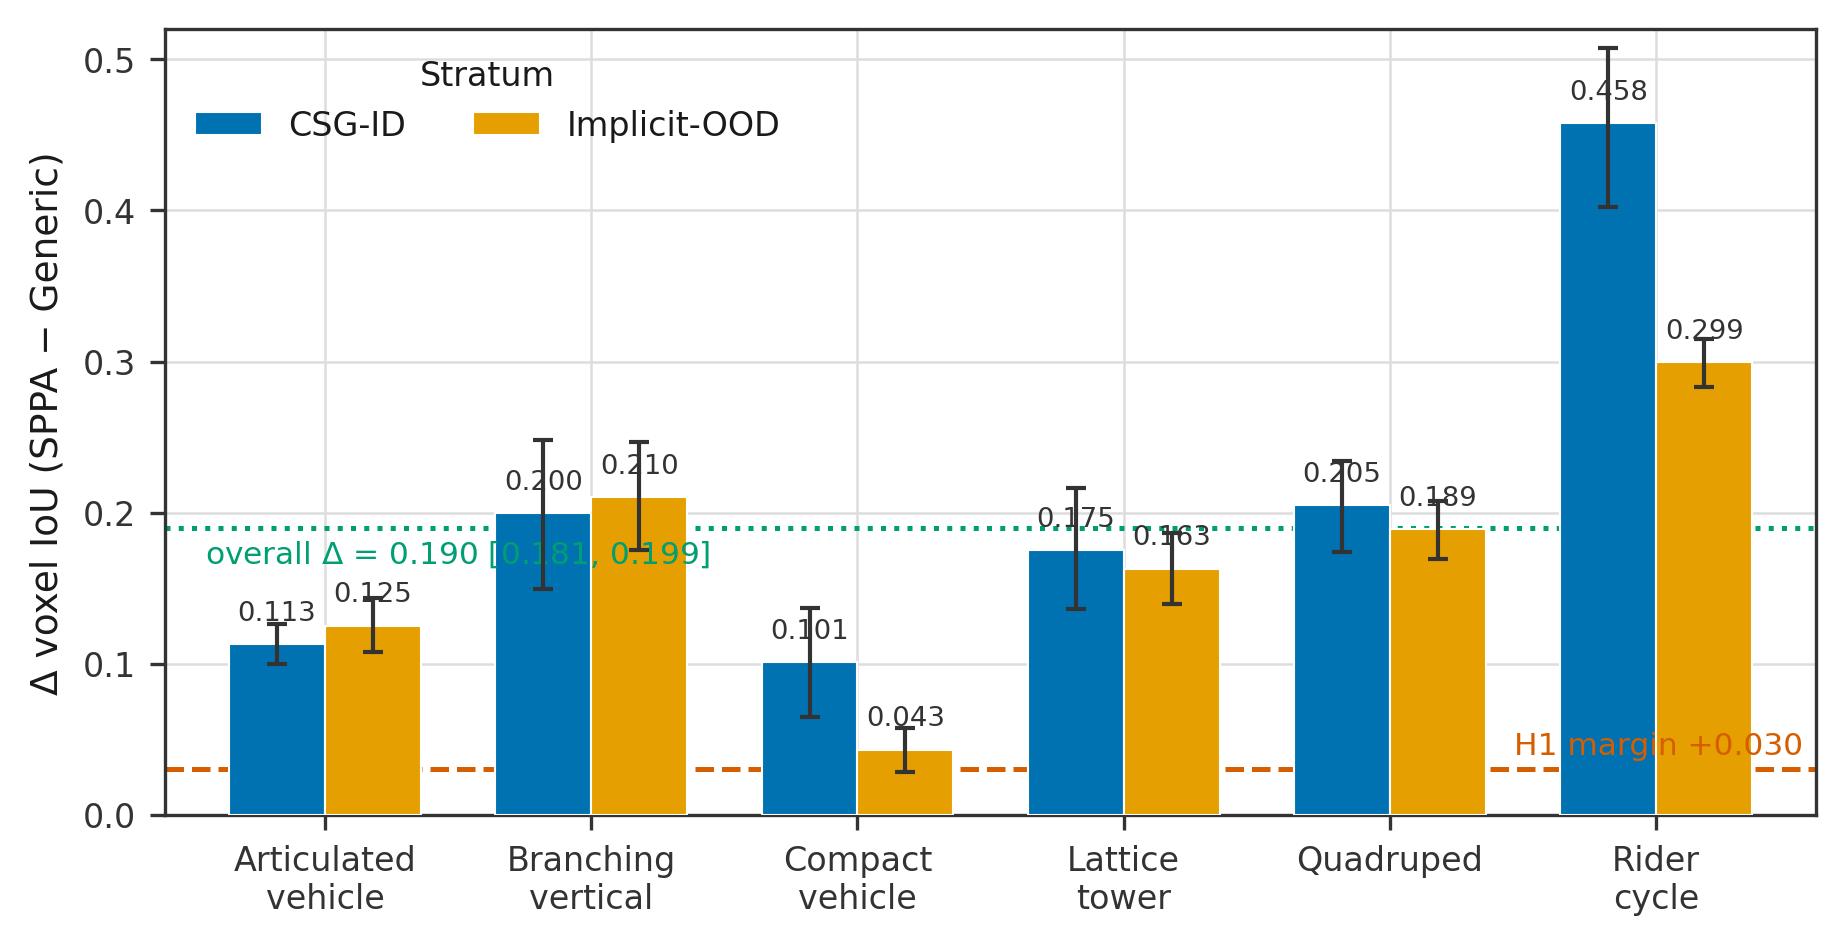
\includegraphics[width=0.55\linewidth]{figures/fig_h1_by_family.png}
\caption{Paired clean-mask mean IoU difference of SPPA minus
Generic graph by morphology family and source stratum (\(n{=}240\)). The
equal-stratum aggregate is the primary estimate of
Table~\ref{tab:mvfit-h1}.}
\label{fig:h1-by-family}
\end{figure}

\begin{table}[!htb]
\centering
\footnotesize
\caption{Paired SPPA minus Generic graph mean IoU difference by
morphology family and source stratum (preregistration \S6 obligation;
\(n{=}20\) actors per cell). Point estimates are sealed
(\texttt{confirmatory\_summary.json}); the per-cell 95\% CIs are NEW post-hoc
within-cell bootstrap intervals (10{,}000 resamples, seed 77157, percentile).
The aggregate row is the sealed primary estimate; the drop-one-family range
is post-hoc and not sealed.}
\label{tab:family-stratum}
\input{benchmarks/results/per\_family\_stratum\_table.tex}
\end{table}

Table~\ref{tab:paired-deltas} reports the sealed paired
differences of SPPA against every baseline under the same stratified
bootstrap construction (method means and wall-clock costs in
RP). SPPA exceeds its text-only ablation (mean
\(\Delta=0.130\), CI \([0.116,0.144]\); the preregistered
\texttt{curated\_family\_tem\-plate} row is this identical method,
deduplicated under Amendment~01) and all lightweight geometric baselines. The margin over the
strongest baseline is much smaller than the headline: the sealed paired
advantage over the nonsemantic visual hull~\cite{laurentini1994visual} is
\(+0.036\) (CI \([0.027,0.044]\)), roughly one fifth of the \(+0.190\)
headline, and visual hull is denser occupancy geometry without a
role-labeled lightweight actor contract, so it is not presented as a
defeated runtime competitor. The summary statistics invert by construction:
the hull's median (\(0.567\)) exceeds SPPA's (\(0.563\)) while its
mean (\(0.522\)) is lower---the paired mean
advantage is carried by a right tail of actors where the eight-part
contract substantially out-fits the hull. Median single-call descriptive
SPPA time is \(9.4\)~ms (p95 \(10.6\)~ms), below the secondary
local-cost gates of 100~ms median / 250~ms p95; under the identical
31-candidate budget the SPPA median fit (\(9.43\)~ms) is slightly
lower than Generic graph's (\(11.34\)~ms), a wall-clock difference the
package records without attributing it to a single cause. A
resolution-sensitivity check
at grids 48/64/80 on the prespecified actor subset changes the paired
difference by at most \(0.0094\), below the \(0.015\) protocol threshold.
Secondary intervals are unadjusted per-comparison intervals; confirmatory
inference is H1 only (Holm-adjusted p-values in RP).

\begin{table}[!htb]
\centering
\footnotesize
\caption{Sealed paired differences of SPPA against every baseline on
the held-out test (clean 64-cubed voxel IoU, \(n{=}240\), stratified
bootstrap, 10{,}000 resamples, seed 77157; all deltas sealed in
\texttt{confirmatory\_summary.json}). Means and medians are recomputed
read-only from the sealed \texttt{raw\_metrics.csv}. Row labels are display
aliases for the preregistered protocol arms \texttt{sppa\_mvfit},
\texttt{sppa\_text\_only}, and \texttt{generic\_mvfit}.}
\label{tab:paired-deltas}
\input{benchmarks/results/paired\_deltas\_table.tex}
\end{table}

\subsection{Robustness to degraded observations (preregistered conditions)}
\label{sec:robustness}

The mission premise is a weak signal---the observation that reaches the twin
may be noisy, partially occluded, or morphologically inconsistent with the
family prior---and this arm measures exactly that regime. The observation
conditions---mask corruption, partial occlusion, and mild and moderate
morphology corruption---were prespecified in the protocol; the inference
over the sealed data is post-hoc under Amendment~04
(Table~\ref{tab:robustness-conditions};
Figure~\ref{fig:robustness-conditions}).
The contrast between corruption types is the headline:
mask corruption costs the paired difference only \(\approx\)\(0.001\) IoU
(\(0.189\) against \(0.190\) clean) and partial occlusion the same
(\(0.189\)); mild morphology corruption leaves the delta at \(0.163\), and
only the moderate level---evidence that
contradicts the graph prior---cuts it to \(0.118\) (CI \([0.106,0.131]\)),
still far above the prespecified \(+0.030\) margin: missing or noisy
evidence is nearly free for this method, and only contradictory evidence
degrades it.

\begin{table}[!htb]
\centering
\footnotesize
\caption{Robustness of the primary comparison to degraded observations
(post-hoc analysis of the sealed confirmatory data under the preregistered
conditions; \(n{=}240\) per condition). Method means and paired differences
under the five prespecified observation conditions. The prespecified
\(+0.030\) margin is exceeded under every condition. Per-condition means of
all eight methods are in RP.}
\label{tab:robustness-conditions}
\begin{tabular}{@{}lrrrr@{}}
\toprule
Condition & SPPA & Generic graph & $\Delta$ paired & 95\% CI \\
\midrule
Clean & 0.557 & 0.367 & 0.190 & [0.181, 0.199] \\
Mild morph. & 0.512 & 0.349 & 0.163 & [0.152, 0.173] \\
Moderate morph. & 0.418 & 0.299 & 0.118 & [0.106, 0.131] \\
Partial occl. & 0.545 & 0.355 & 0.189 & [0.179, 0.200] \\
Mask corrupt. & 0.555 & 0.367 & 0.189 & [0.179, 0.197] \\
\bottomrule
\end{tabular}

\end{table}

\begin{figure}[!htb]
\centering
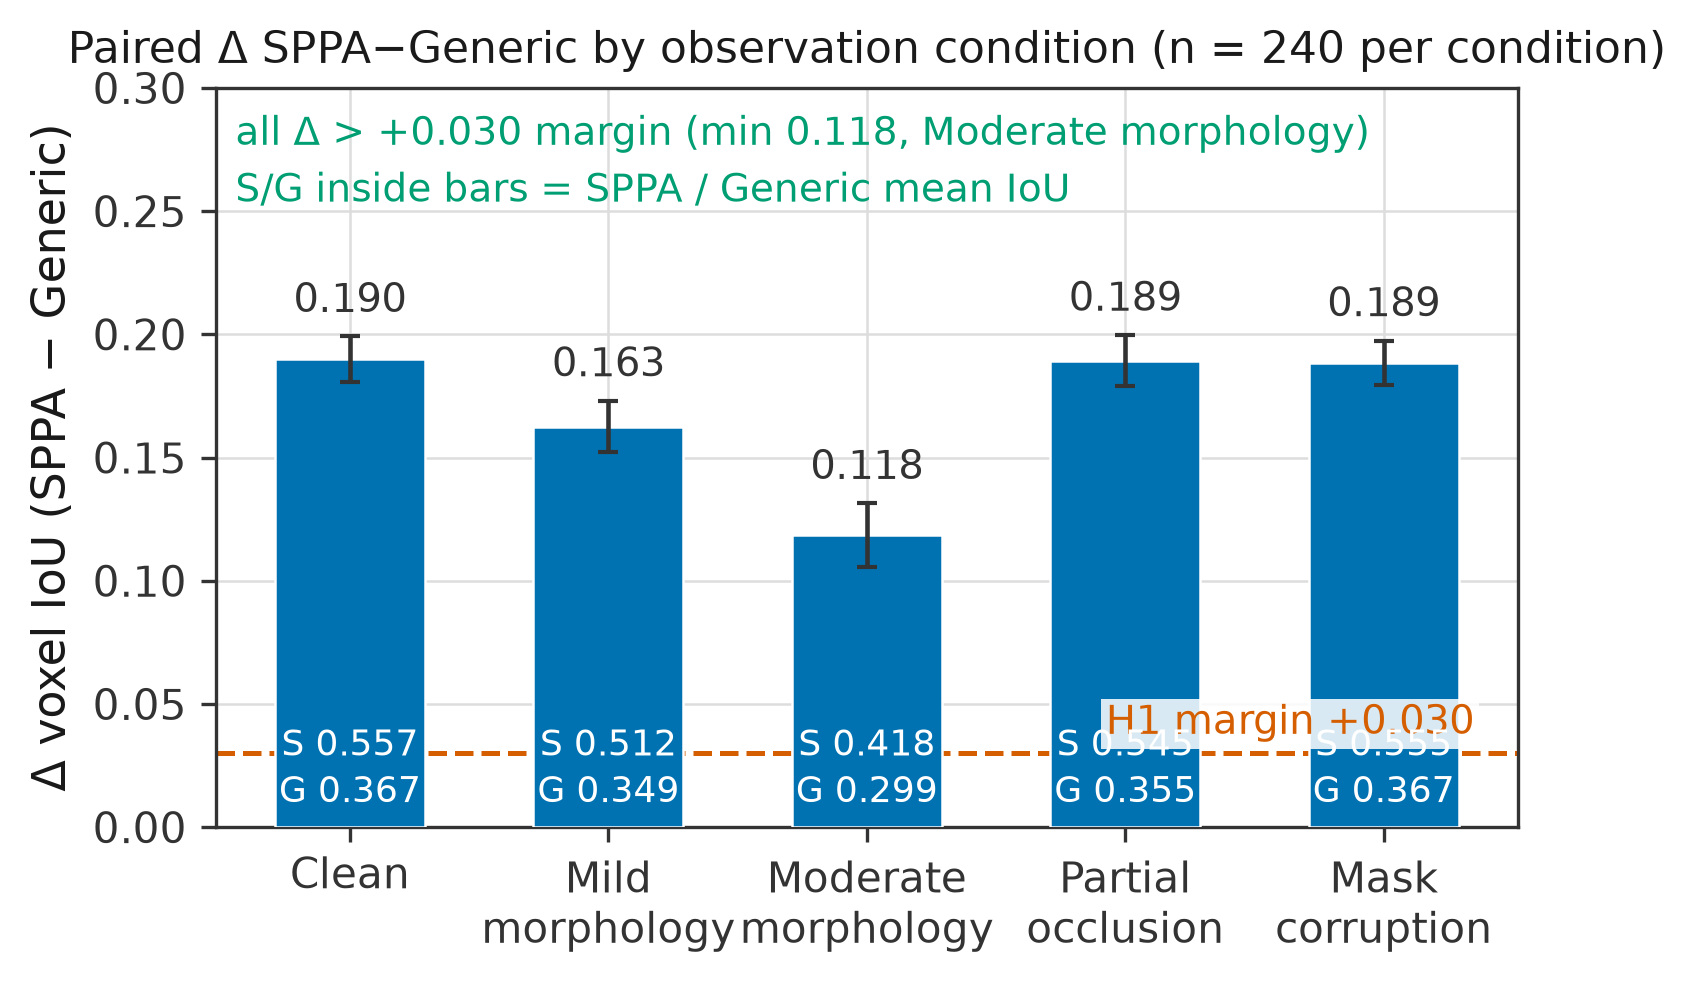
\includegraphics[width=0.55\linewidth]{figures/fig_robustness_conditions.png}
\caption{Paired SPPA minus Generic graph mean IoU difference with 95\%
bootstrap intervals under the five prespecified observation conditions
(\(n{=}240\) per condition). The dashed line marks the prespecified
\(+0.030\) margin.}
\label{fig:robustness-conditions}
\end{figure}

Exactly \(5\) of \(240\) clean cases fall below the prespecified failure
threshold (voxel IoU \(<0.25\)); all five are \texttt{lattice\_tower} CSG-ID
cases whose leg and plate thicknesses sit below the voxel cell, and every
method scores at the floor on them---a resolution effect shared by every
method, not a family-prior failure. Convergence telemetry supports the same
reading: \(88.7\%\) of SPPA cases still improve in the final sweep and
its \(\theta\) never sits at the frozen bounds, whereas Generic graph pins
\(\theta\) at a bound in \(57.9\%\) of cases---evidence of a mismatched
prior, not of SPPA overfitting. Surface metrics agree with the volume
ranking (Chamfer and F-score tables in RP).

\paragraph{Representation versus fitting: graph-by-fitting decomposition.}
\label{sec:results-decomposition}
A post-hoc exploratory analysis completes the graph-by-fitting factorial:
the previously missing cell, the generic
graph at the default \(\theta_0\), scores \(0.180\). The family graph with no
fitting at all (\(0.427\)) already exceeds the fully fitted generic
competitor (\(0.367\)). Fitting adds \(+0.187\) on the generic graph and
\(+0.130\) (CI \([0.117,0.143]\)) on the family graph, with a negative
interaction (\(-0.058\)). The H1 headline therefore decomposes into a larger
representation effect---graph effect at no fit \(+0.248\), CI
\([0.234,0.261]\)---plus a smaller fitting contribution on top of it, and the
claim of this paper is accordingly about the family-conditioned
representation, not about fitter sophistication.

\subsection{Wrong-family tokens}
\label{sec:wrong-family}

The confirmatory benchmark supplies the correct family token, so it does not
measure the principal failure mode of a family-conditioned method. As a
post-hoc exploratory arm, each
held-out actor was therefore also fitted under each of the five incorrect
family tokens (1{,}200 additional deterministic fits through the same fitting
path; Figure~\ref{fig:wrong-family-matrix}). A wrong token is far worse than
no family prior at all: the wrong-token mean is \(0.205\) against
Generic graph \(0.367\), a paired difference of \(-0.162\) (CI
\([-0.167,-0.158]\)), with \(98.3\%\) of actors scoring below their own
generic fit, and even the per-actor \emph{best} wrong token (\(0.361\)) does
not beat the generic mean. The deployed contract already routes unsupported
labels to a generic fallback volume; this result makes the symmetric design
implication explicit---accept a family token only with adequate detector
confidence, and otherwise degrade to the generic graph rather than commit to
a mismatched family.

\begin{figure}[!htb]
\centering
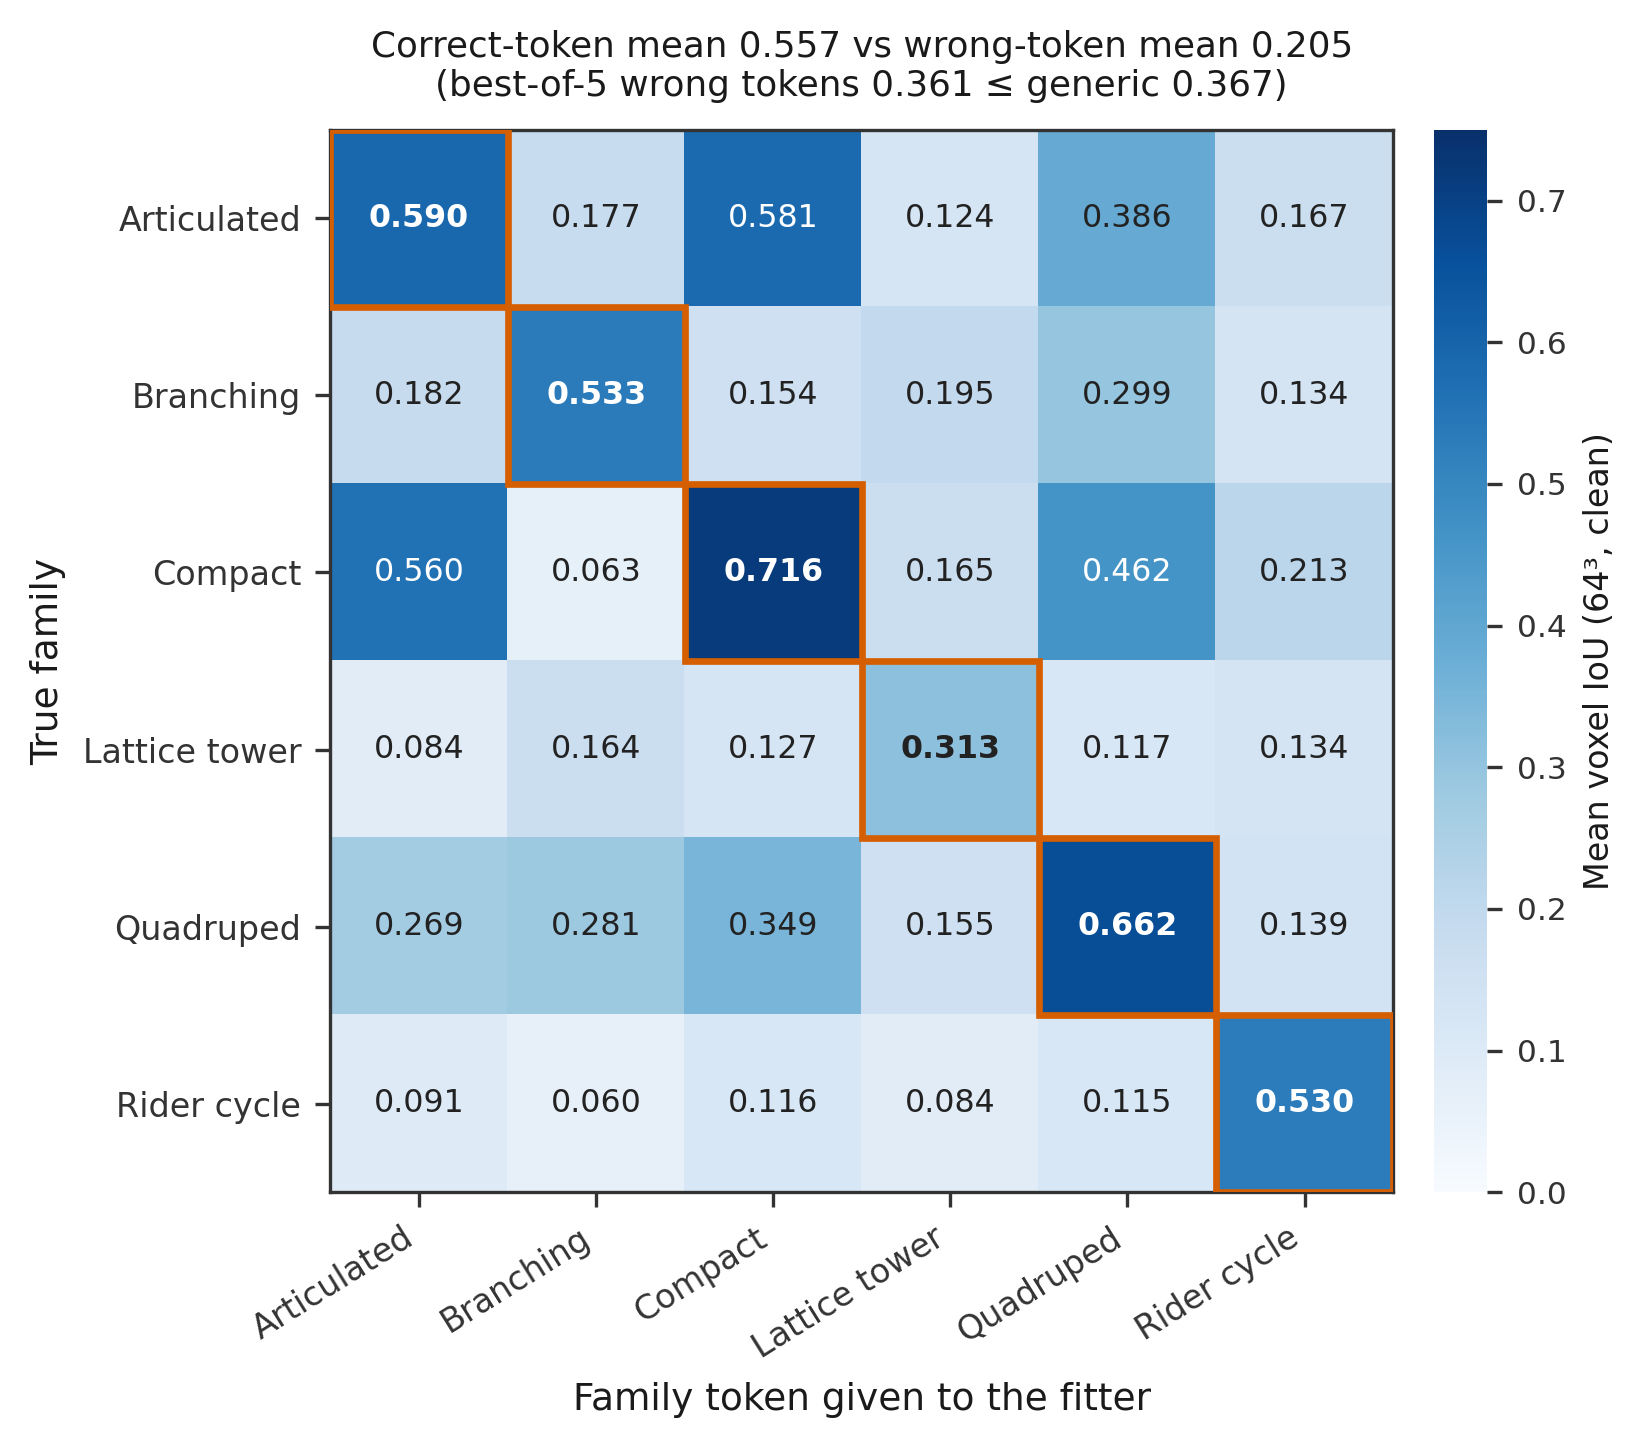
\includegraphics[width=0.55\linewidth]{figures/fig_wrong_family_matrix.png}
\caption{Wrong-family analysis (clean condition, \(n{=}240\), mean voxel IoU).
Rows: true family; columns: family token supplied to the fitter. The diagonal
is the correct token. Off-diagonal cells fall below the diagonal and, with
few exceptions (the morphologically close vehicle families), also below the
generic-graph mean of \(0.367\).}
\label{fig:wrong-family-matrix}
\end{figure}

\subsection{Adversarial family instances}
\label{sec:adversarial}

A structural concern with the primary comparison is that it is nearly
guaranteed: the family graph encodes the same part topology that the CSG-ID
generators instantiate, so a positive H1 could be decided by design rather
than by measurement. The wrong-family arm already shows the prior can be
actively harmful; here we probe the complementary edge. A post-hoc
exploratory stratum of \(120\) adversarial actors (\(20\) per family, twelve
documented violation types, design frozen before measurement) keeps each
family's semantic class but violates its structural prior: rearward cabs,
split cargo beds, six-legged quadrupeds, out-of-order
platforms, a \(25^{\circ}\) leaning lattice tower, sidecar cycles, and
over-scaled cargo. Under the identical clean-mask
protocol, the paired SPPA advantage over Generic graph falls from \(+0.209\)
on the same actors unviolated (i.e., the CSG-ID stratum) to \(+0.141\) (CI
\([0.125,0.157]\)): violating
the prior destroys about one third of the advantage
(\(\Delta\Delta=-0.068\), CI \([-0.087,-0.048]\)) and SPPA loses at
actor level in \(8.3\%\) of cases. Two violation types reach statistical
ties with both methods near the floor---the leaning tower (\(+0.009\), CI
\([-0.008,+0.026]\); a \(25^{\circ}\) shear is not expressible by
axis-aligned part scaling) and the cascade crown (\(+0.007\), CI
\([-0.015,+0.029]\))---while others leave the advantage intact or larger
(sidecar \(+0.320\)). The family prior is therefore neither a tautological
win nor a fragile one: its value degrades measurably with
prior violation (table in RP).

\subsection{Ablations and sensitivity analyses}
\label{sec:ablations}

\paragraph{Generic-graph design sensitivity.}
\label{sec:generic-sensitivity}
Because the authors designed the generic graph (Section~\ref{sec:mvfit}),
three alternative generic graphs were registered in writing before any
measurement and evaluated under the same protocol: G2 (box/cylinder chassis),
G3 (vertical ellipsoid stack plus legs), and G4 (slot-wise mean of the six
family graphs, a fully mechanical rule). All three score \emph{below} the
original generic (table in RP): the measured SPPA advantage is, if anything,
conservative.

\paragraph{Part-query task.}
To operationalize what role labels are worth, a part-query task was frozen in
writing before measurement on the same stratum: given a target role
(\emph{cargo}, \emph{wheels}, \emph{cab}, \emph{legs}, \emph{hitch},
\emph{platforms}), each method must return the voxels of that part. Controls
are the Generic graph baseline with its own slot mapping and two frozen visual-hull
heuristics (largest connected component; lower half). Over 887 scorable
queries (33 of 920 excluded for sub-voxel ground truth, with a sensitivity
analysis), SPPA reaches
query F1 \(0.434\) versus \(0.145\) (generic), \(0.111\) and \(0.087\) (hull
heuristics), with normalized part-centroid error \(0.055\) versus
\(0.177\)--\(0.249\); the hull \emph{covers} (recall \(0.96\)) but cannot
\emph{select} (precision \(0.07\)). Structural part counting is exact in
\(70\%\) of actors versus \(0\%\) for the hull (table in RP).

\subsection{External sanity check on real meshes}
\label{sec:external-sanity}

As a post-hoc exploratory case study outside the design distribution, the
same methods were run on \(n{=}52\) real third-party meshes (Objaverse LVIS
subset and ModelNet40), mapped to the six families through a class-to-family
mapping frozen in writing before any evaluation (full table, per-case
scatter, and a qualitative gallery in RP). Mean fit
time remains millisecond-scale (\(9.8\)~ms per case, CPU); the sample is
small, the class mapping approximate, and the evaluation reuses the
synthetic-grid protocol on real geometry---a sanity check, not a benchmark.

Three readings follow. First, the preregistered margin does not replicate on
external meshes at this sample size: SPPA scores \(0.413\),
CI \([0.359,0.467]\), against Generic graph \(0.370\), CI \([0.335,0.405]\), a
paired \(+0.043\) whose interval \([-0.007,+0.094]\) includes zero---at
\(n{=}52\) the interval resolves only large effects. Second,
the nonsemantic visual hull dominates raw occupancy with clean real
silhouettes (\(0.656\), CI \([0.606,0.704]\)), and the trivial geometric
primitives tell the same story: capsule (\(0.492\)), ellipsoid (\(0.485\)),
and even the axis-aligned box (\(0.411\)) match or exceed SPPA
(\(0.413\)) here---outside the design distribution the family graph buys no
volumetric advantage over shape-free baselines, and the value of SPPA is the
semantic contract: role labels, bounded updates, and a telemetry-scale
payload (the coverage-without-selection regime priced by the part-query
task, Section~\ref{sec:ablations}).
Third, the failure modes are informative and consistent with
Section~\ref{sec:wrong-family}: template--instance mismatch (horizontal water
towers fitted by a vertical tower graph), open geometry (bicycle wheel
spokes), and one LVIS mislabel retained as an out-of-distribution case (a
giraffe labeled \texttt{horse}). When the prior does not match, it hurts; the
contract's role is to detect that situation and degrade safely.

\subsection{External neural generators: an input-modality mismatch demonstration}
\label{sec:neural-external-wave}

A secondary analysis, specified in writing before any measurement, compares
SPPA with four measured external neural image-to-3D generators,
TripoSR~\cite{tochilkin2024triposr}, Hunyuan3D-2mini-turbo and the flagship
Hunyuan3D-2 full model~\cite{zhao2025hunyuan3d}, and
TripoSG~\cite{triposg2025}, on sixty of the held-out cases, each under two
inputs: a clean-crop shaded oblique render, its best condition, and the raw
\(96\times96\) top telemetry mask, the closest visual analog of the channel
SPPA consumes (full table, Pareto figure, and protocol in RP). On these cases
SPPA reaches \(0.561\) mean voxel IoU at \(9.2\)~ms CPU with a
\(1.45\)~kB update descriptor, against \(0.128\)--\(0.231\) for the measured
neural outputs over seven of the eight method-by-input conditions---the
eighth, TripoSG on the raw mask (\(0.002\)), is the input-parity artifact
registered in RP and excluded from this range---whose meshes carry
\(28\)k--\(3.4\)M triangles and MB-scale payloads on an RTX~5090. Every
generator with a parity-clean input comparison scores \emph{higher} from the
harsh top mask than from its generous clean-crop render: single-view
image-to-3D models hallucinate occluded structure, whereas a calibrated
footprint constrains occupancy directly, so in this asymmetric setting
telemetry-shaped evidence behaves not as a degraded image but as a different
measurement channel. The wave measures one operating point per system under
deliberately asymmetric input channels, not an image-to-3D leaderboard; the
flagship Hunyuan3D-2 full model (\(0.148\) oblique, \(0.177\)
mask) sits inside the same band as its distilled mini/turbo variant,
retiring the distilled-checkpoint caveat.

\subsection{Real-image probes and deployment runtime}
\label{sec:deployment-summary}

Real-image probes exercise the dual-input contract of
Section~\ref{sec:pipeline}: a YOLOE-26s
open-vocabulary detector supplies approximate semantic evidence on the image
path, while the tag path uses reviewed text only. Detector evidence is not
treated as ground truth: weak labels are refined only to conservative
families, implausible footprint aspect ratios are clamped by family priors, and
unsafe image-derived pose is withheld from the runtime descriptor.
Two real flight photos recorded for this paper (2026-07-21) run the full
chain end to end (Figure~\ref{fig:real-flight-probes}). The tower photo
receives \texttt{electric pylon} (confidence \(0.49\), 38-point native mask)
and enters the \texttt{power\_tower} family: the geo-projected mask footprint
(\(39.9\times17.5\)~m, cables included) is implausible for a tower, so the
gate clamps it through the vertical-structure aspect prior to
\(5.60\times5.60\times28.00\)~m (396-triangle lattice
proxy). The tractor photo is mislabeled by the detector as
\texttt{two-wheeled vehicle} (\(0.48\)), so it is routed to the conservative
\texttt{generic\_vehicle} family rather than a committed wrong token; the
\(7.1\times6.0\)~m footprint is fused to \(4.75\times2.50\times2.60\)~m
(576-triangle proxy). On the same crops and workstation, six measured neural
generators run at
their fastest official configurations WITH official background removal
(Figure~\ref{fig:real-flight-probes}):
SF3D and TRELLIS.2 even recover the tower lattice, but every generator
costs orders of magnitude more than the SPPA proxies built from the same
evidence in milliseconds on CPU with no GPU, and Hunyuan3D-2mini
returns no surface on the two real aerial crops (per-case values
in RP). Telemetry
for these replays is declared assumed flight
(\(45\)/\(35\)~m AGL, nadir camera), not measured, and no 3D ground truth
exists, so this fidelity reading is qualitative and no IoU is
reported. Further archived probes, replay audits, input-mode
ablations, a verifier-gated open-label probe of 20 awkward labels (\(8/20\)
recipes verified, zero critical mismatches), and a role-preservation
diagnostic are retained in RP.

The deployment layer is the descriptor/update contract consumed by the
optional Unreal Engine 5.7 backend. Table~\ref{tab:deployment-runtime-summary}
condenses the runtime evidence (full Unreal/HISM run matrix in RP). Packaged
replay at 100 synthetic objects passes a
33.3~ms desktop frame budget but misses 60~FPS; dense shape updates remain the
limiting factor even under HISM batching, and curated assets remain preferable
when a matched asset exists (shape-stream P95 \(6.789\)~ms vs.\ \(22.445\)~ms
on the cow/tower subset). The deployment claim is therefore scoped to the
regime the mission actually presents---sparse field scenes with tens of
concurrent dynamic objects, 30~FPS-class rendering---not to dense urban
object counts: at 500 densely updated objects the HISM shape path exceeds the
frame budget by more than five times (Table~\ref{tab:deployment-runtime-summary}).

\begin{table}[!htb]
\centering
\footnotesize
\setlength{\tabcolsep}{3pt}
\renewcommand{\arraystretch}{1.12}
\caption{Deployment runtime evidence, split by evidence tier: measured
on real or recorded data (top) and packaged synthetic replays used for the
scaling limits (bottom; full run matrix in RP). Python contract timings are
not Unreal frame times.}
\label{tab:deployment-runtime-summary}
\begin{tabularx}{\linewidth}{@{}L{0.44\linewidth}Y Y@{}}
\toprule
Evidence & Value & Note \\
\midrule
\multicolumn{3}{@{}l}{\emph{Measured on real or recorded evidence}} \\
Fit latency on the recorded real stream (Section~\ref{sec:real-stream}) & \(11.8\)~ms median & 2--15~Hz stream \\
Measured JSON update traffic (no-ops suppressed) & 25.8--37.4~kB/s & per-object update messages on the recorded stream \\
\midrule
\multicolumn{3}{@{}l}{\emph{Packaged synthetic replays (scaling evidence, not live flight)}} \\
Python contract build (descriptor + update + scheduler) & P95 \(\leq 0.52\)~ms & contract cost \\
Editor-Cmd and packaged recorded replay & 27/27 payloads accepted & recorded streams \\
Packaged 100-object replay, pose/shape frame P95 & \(17.8/19.3\)~ms & misses 60~FPS P95 \\
HISM dense updates, 100/250/500 objects, shape frame P95 & \(37.1/94.0/186.1\)~ms & over the 33.3~ms budget \\
HISM partial update, 500 objects (10\% changed tracks) & pose/shape P95 \(16.5/29.8\)~ms & synthetic schedule \\
\bottomrule
\end{tabularx}
\end{table}

\subsection{A real detector stream case study}
\label{sec:real-stream}

As a post-hoc exploratory case study whose value is its degraded
signal, a recorded 1{,}394-frame
flight
stream over the Ejea twin was re-analyzed end to end: a custom YOLO detector
with real confusions (cows hallucinated on tower
textures), MAVLink telemetry, and exact simulator ground truth for the
static tower anchors. Detections with locked telemetry yield 1{,}902 cases
(308 tower, 848 cow, 746 biker detections). Every method receives the
identical observation---an oriented ground footprint geo-projected from the
detection box plus a monocular height estimate---so the comparison carries
no input advantage, and wrong detector tokens are kept as a natural
condition (RP).

Three findings characterize the degraded-signal operating point, and we
report them in the order a critical reader will check them
(Table~\ref{tab:real-stream}; Figure~\ref{fig:real-stream}). \emph{First, the
headline inverts on real evidence.} SPPA does \emph{not} win the only metric
this stream can score---2D reprojection overlap---against any nonsemantic
baseline (\(0.298\) median versus \(0.423\) for Generic graph and
\(0.44\)--\(0.45\) for OBB, visual hull, and capsule), and the oriented box
does so at \(0.22\)~ms, roughly fifty times cheaper than our \(11.8\)~ms
fit. We do not explain this away: the monocular height estimate genuinely
conflicts with the family prior bounds (a \(13.75\)~m tower column versus a
\(\approx\)\(5\)~m observed extent), the 2D metric structurally favors
shape-free footprints, and the stream carries no 3D ground truth, so the
part-structure advantage SPPA is built for cannot be scored here. The honest
reading is that on real degraded evidence the family prior buys 3D part
structure at a measurable 2D price, and whether that price is worth paying
is a decision the system must make per detection---which is exactly what the
third finding operationalizes. \emph{Second, the evidence-versus-prior
tension is quantifiable and diagnostic.} On the 138 GT-matched cases where
the real detector emitted a wrong family token, refitting with the correct
token collapses the 2D fit from \(0.381\) to \(0.025\): the correct prior
cannot explain the misleading evidence that triggered the wrong label
(token-arm table in RP). A ground-truth benchmark cannot see this tension;
the stream can. \emph{Third, the operating point is computationally viable
and trust is measurable}: fit latency (\(11.8\)~ms median) stays far below
the 2--15~Hz stream rate, and the token-validation signals below turn the
first finding into a measured routing decision. Localization is outside this
paper's scope: all methods share the same \(\approx\)\(33\)~m median 3D
error, set by the monocular observation geometry (full analysis in RP).

\paragraph{Token validation and trust-gated routing (post-hoc).}
The same stream provides a measured token-validation signal (protocol frozen
before any outcome; ROC in RP):
on the 217 GT-matched cases,
\(-\)confidence separates the 138 wrong-token from the 79 correct-token cases
with AUC \(0.847\) (95\% CI \([0.792,0.898]\)). Prior mismatch separates
them perfectly on this stream (AUC \(1.000\))---we flag this number rather
than celebrate it: it arises in the direction opposite to intuition, because
cow/biker hallucinations receive small monocular heights that fit their
wrong family priors suspiciously well while true towers suffer severe
monocular height underestimation
(\(\approx\)\(5\)~m observed against a \(25\)~m prior). With \emph{no
observed overlap} between groups, this is a stream-specific artifact of one
detector's failure mode, not a population claim, and we do not expect it to
transfer; the \(0.847\) confidence signal is the transferable one. A frozen
routing policy on these signals
(registered 2026-07-19 before any outcome; RP) turns the signal into a
measured coverage decision---and this policy, not the raw fit, is the
section's operational result:
routing detections below confidence \(0.34\) to the nonsemantic proxy
fallback lifts the stream-level median 2D IoU from
\(0.298\) (always-SPPA) to \(0.432\) (\([0.427,0.435]\)) while still
compiling the \(19\%\) most confident detections into family proxies.
Family conditioning and shape-free fallback are thus not competitors but a
single gated system: commit the semantic prior where it is trusted, degrade
gracefully where it is not.

\paragraph{A first real-video pass (exploratory post-hoc).}
A 23.9-s segment of real onboard flight video (239 frames at 10~Hz, cut by
the operator from the M\_20\_1RR sortie of 2026-07-06, with synchronized
ArduPilot telemetry) yields 147 YOLOE-26s detections; tower-class
hypotheses appear in 99/239 frames (median confidence 0.31, best 0.58),
and the pylon's bounding box grows coherently as the drone closes in.
Metric evaluation against four PNOA-georeferenced lattice poles
(\(\approx\)1--2~m accuracy) is deferred---the camera mount is not
calibrated---so this arm reports real
detection evidence only, not metric accuracy.

\begin{table}[!htb]
\centering
\scriptsize
\setlength{\tabcolsep}{3pt}
\caption{Real detector stream case study (exploratory post-hoc, not sealed):
1{,}902 detections from a 1{,}394-frame flight over the georeferenced twin
with a real custom detector, real telemetry, and exact tower-anchor ground
truth. Localization
and footprint columns (GT-matched subset, \(n{=}217\)) are retained in RP.
SPPA trades 2D image
overlap for 3D part structure (the stream has no 3D ground truth).}
\label{tab:real-stream}
\begin{tabular}{@{}lcc@{}}
\toprule
Method & 2D reproj. IoU med. [P25, P75] & Latency (ms) \\
\midrule
SPPA (this work) & 0.298 [0.218, 0.392] & 11.8 \\
Generic graph & 0.423 [0.394, 0.448] & 13.4 \\
OBB & 0.446 [0.398, 0.492] & 0.22 \\
AABB & 0.330 [0.299, 0.357] & 0.25 \\
Visual hull (non-semantic) & 0.446 [0.398, 0.493] & 0.50 \\
Capsule & 0.445 [0.422, 0.466] & 1.31 \\
\bottomrule
\end{tabular}
\end{table}

\begin{figure}[!htb]
\centering
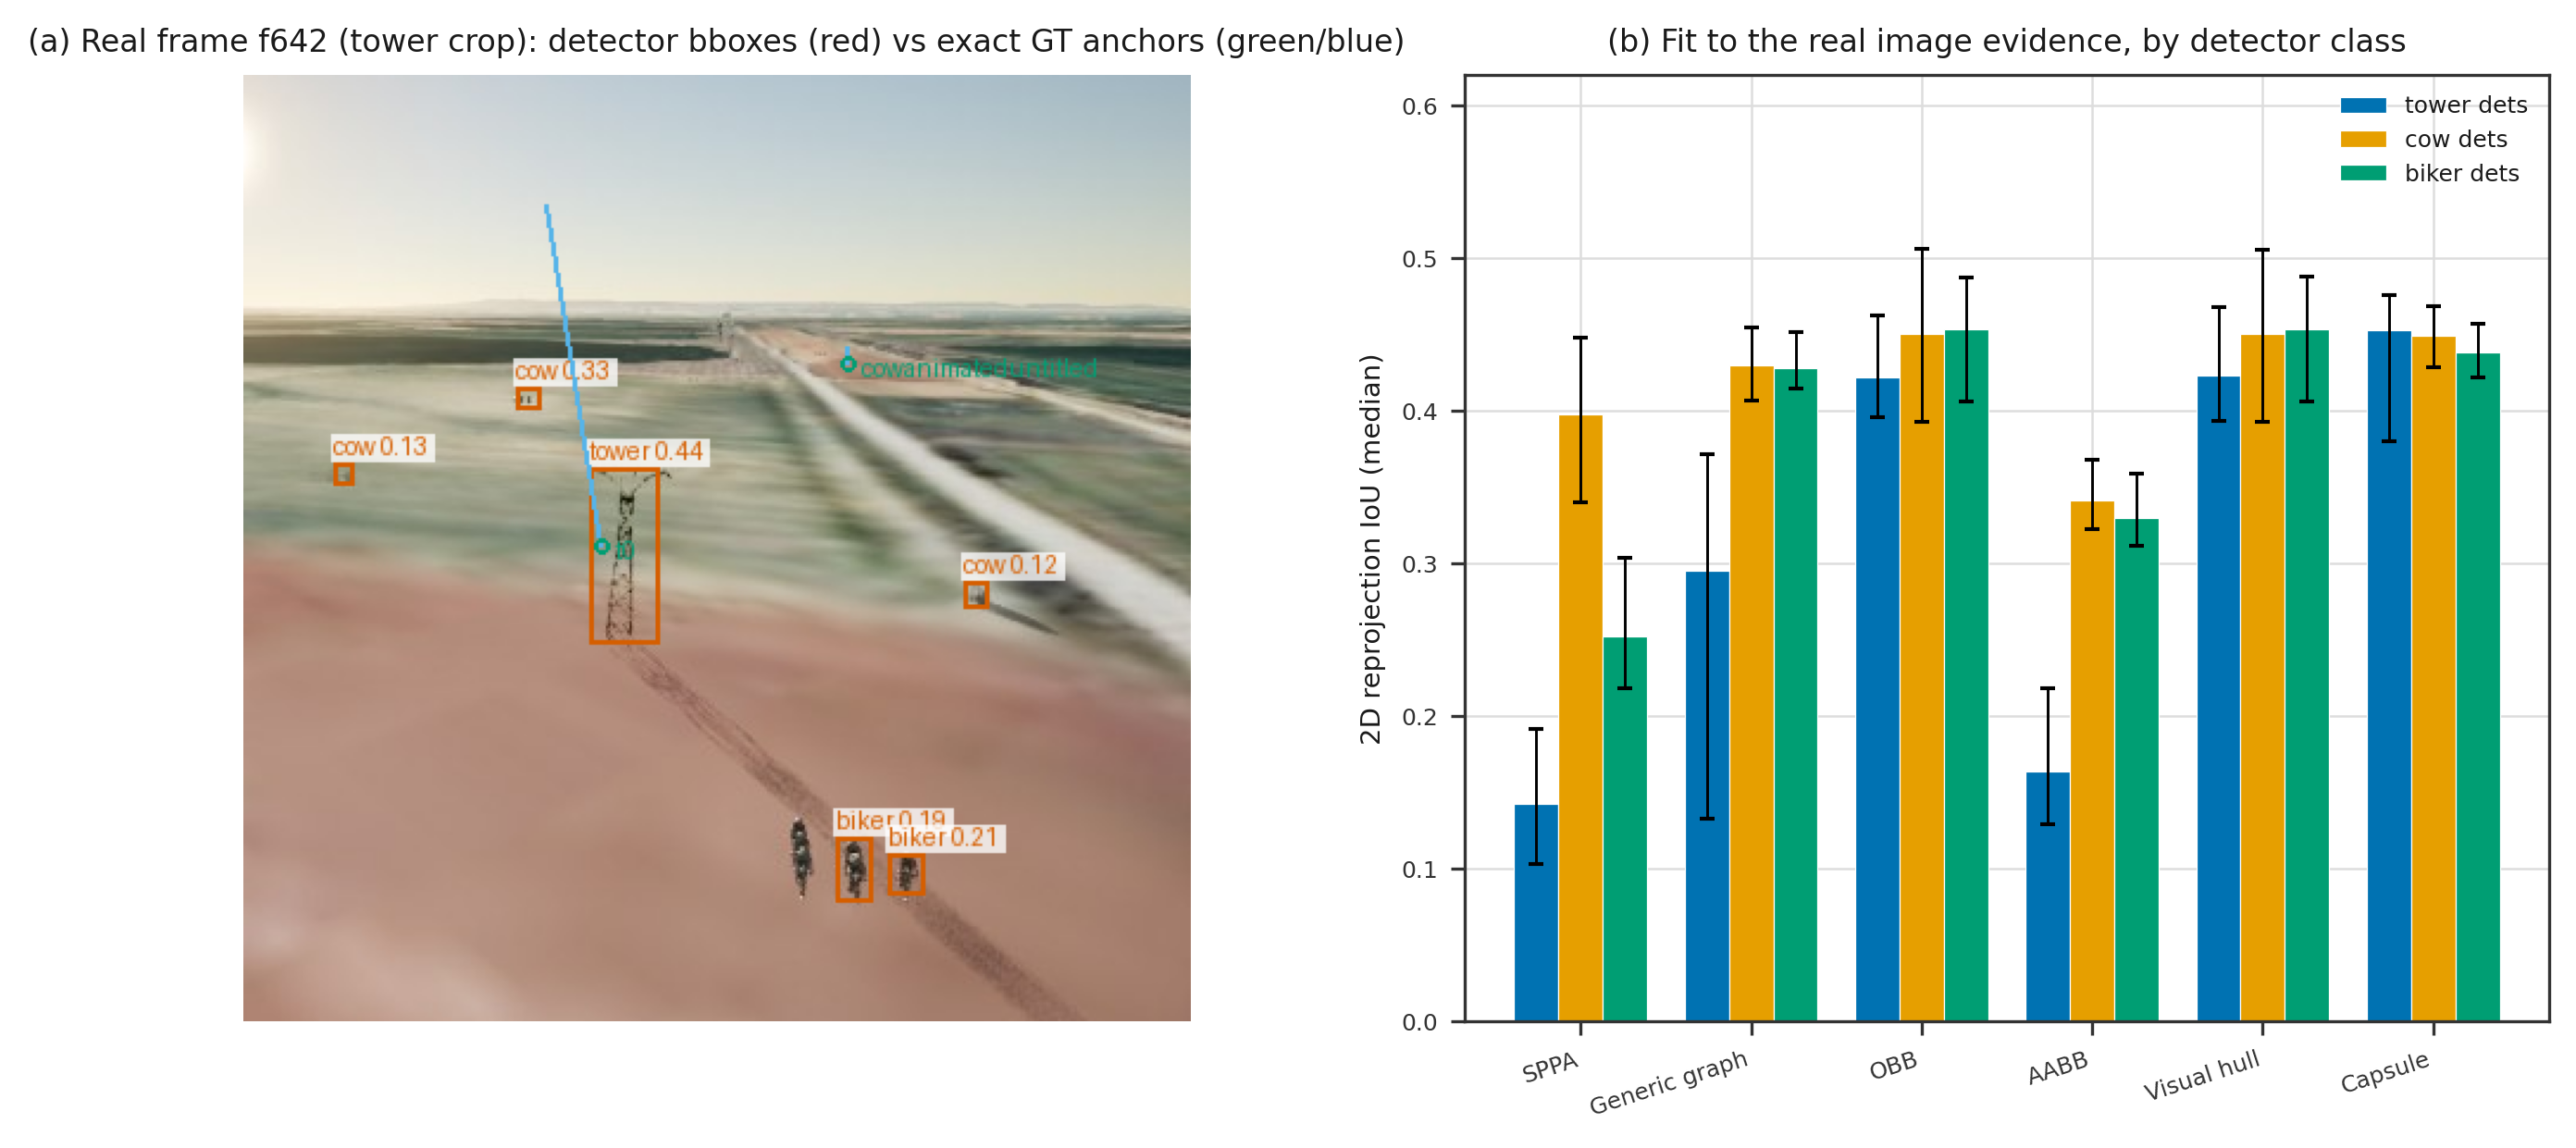
\includegraphics[width=0.55\linewidth]{figures/fig_real_stream_main.png}
\caption{Real stream case study, degraded-signal view. (a)~Frame 642
(tower crop) with
detector boxes and exact ground-truth anchors reprojected through the same
camera model. (b)~2D reprojection IoU against the real image evidence, by
detector class: SPPA does not win this 2D metric; the family prior
buys 3D part structure instead.}
\label{fig:real-stream}
\end{figure}

\section{Discussion}
\label{sec:discussion}

The confirmatory result answers the preregistered question behind the
stale-twin delta mission: under identical calibrated
silhouettes and optimizer budget, a frozen family part graph improves
lightweight occupancy over a generic eight-part graph by a large and stable
margin, and the decomposition attributes most of the advantage to the
representation rather than to the fitter. The margin holds under
every preregistered observation corruption, although the degraded-sensing
evidence combines synthetic corruptions, simulated demonstrations, and one
recorded stream---no hardware measurement of
degraded operation exists. Read together, the evidence supports a sharper
thesis than the headline alone: \textbf{a family-conditioned prior is an
asset only inside a measured trust envelope, and the envelope is as much the
contribution as the prior.} The boundary analyses define that envelope: a
wrong family token is worse than no prior at all, making fallback routing a
measured requirement;
adversarial violations of the structural prior destroy a measurable share of
the advantage; on external real meshes the margin does not
replicate at this sample size, where what remains differentiating is the
contract---role labels, bounded updates, and a telemetry-scale payload, with
the part-query value that dense occupancy baselines cannot
select---rather than volumetric leadership; and on the real detector stream
the prior loses the 2D metric outright while the trust-gated routing policy
recovers the stream-level operating point (\(0.298\to0.432\) median 2D IoU).
A twin layer that knows when \emph{not} to use its own prior is the system
property we argue the dynamic-object literature is missing; the measured
signals that gate it (detector-token confidence and prior fit) are provided
by this paper; two further exploratory
simulated-twin studies
(cross-view reconstruction fidelity and camera-less simulated-LiDAR sensing)
are retained in RP.

The contract also supports the temporal regime a real sortie implies:
because one build costs milliseconds, an actor can be re-fitted as often as
evidence
improves, so the proxy
\emph{converges} over the approach instead of being committed at first
sight; the measured token-validation signals of
Section~\ref{sec:real-stream} are the trust signal that should gate such
refinement, and per-part bounded refinement within role-declared limits is
the natural next rung of this ladder, left to future work.

\label{sec:threats}Four threats to validity remain binding.

\begin{itemize}
\item \emph{Design and estimand.} The primary comparison is structurally
favored by design---the family graphs encode the same part topology that the
CSG-ID generators instantiate---so preregistration quantifies the effect but
cannot make it surprising. The implicit-OOD stratum keeps a
\(0.172\) margin, and the boundary map (wrong-family,
adversarial, external meshes, real stream) carries the rest of the
load-bearing evidence, not H1 alone. The same
team authored the family graphs and the generic competitor; the sensitivity
variants of Section~\ref{sec:generic-sensitivity} bound, but do not
eliminate, the resulting baseline-design risk.
\item \emph{Data.} The held-out set is synthetic and developer-held-out;
OOD-stratum differences do not license claims about real UAV masks,
detectors, or metric flight geometry. Family tokens are supplied, so the
experiment is family-conditioned rather than open-set, and silhouettes are
clean orthographic projections plus prespecified corruptions, not real
detector masks. Deployment coverage is family-level: the detector runs an
operator-frozen prompt list, aerial
mislabels are routed conservatively (measured:
tractor\(\to\)\texttt{two-wheeled vehicle}), and an unmapped label becomes
the generic uncertainty volume rather than a fitted proxy.
\item \emph{Sensors and twin studies.} The camera is the validated sensor:
LiDAR interchangeability and night, fog, or smoke operation are evaluated
only through the prespecified synthetic corruptions and exploratory
simulated-twin demonstrations (retained in RP; post-hoc, not confirmatory),
not measured on hardware or in degraded weather.
\item \emph{Runtime and stream.} ``Instant'' is per object (millisecond
median fit, local CPU wall-clock, not flight-laptop frame time); dense
packaged shape updates do not reach 60~FPS and remain the
declared limiting factor, and packaged replays are short synthetic streams. The
real-stream study is one recorded flight with one custom detector,
no 3D ground truth, and 2D reprojection metrics only;
its measured operational signal is token validation (AUC \(0.847\)
\([0.792,0.898]\) for \(-\)confidence; \(1.000\) for \(-\)prior-mismatch on
217 matched cases---no observed overlap, not a population
claim).
\end{itemize}

The supported claim is deliberately narrow, and we treat that narrowness as
the design principle rather than an apology: family conditioning
improves occupancy beyond the prespecified margin on the held-out synthetic
test, SPPA descriptors are consumable by an optional Unreal backend, and the
trust envelope around the prior is itself measured;
real-UAV accuracy, universal open-set geometry, operator benefit, and neural
image-to-3D ranking remain outside the claim---each excluded because the
evidence presented here does not measure it, and each convertible into a
claim only by the experiments below.
Four directions are left to future work, each tied to a gap this paper
measured rather than to generic outlook. First, the frozen coordinate-descent
fitter could be replaced by population-based or differentiable-rendering
fitting, or amortized by a small learned
mask-to-\(\theta\) predictor, keeping the representation and contract. Second, the external gap measured
here---non-replication on 52 real meshes, the inverted 2D metric on the real
stream---calls for public real-data tests with metric ground truth and
detector-derived silhouettes; we consider this the single most valuable
experiment the community could run against this work. Third, the
open-set coverage of the reviewed family library should be climbed beyond
string matching:
an embedding-based label router, per-part bounded
refinement within role-declared limits, and runtime gated schema proposal
(an offline gated-proposal study in RP is the starting point). Fourth, any
operator-facing benefit requires a dedicated human-factors study; the present
paper contains none.

\section{Conclusion}

SPPA targets the moment a UAV digital twin must be updated under a
weak signal: the static layer is stale, the image link does not
suffice, and the detections that do arrive must become explicit per-object
volumes at once. This paper has shown three things about that moment. First,
a reviewed semantic part graph is a measurable occupancy prior: the
preregistered equal-budget comparison passes its prespecified margin and
holds under every preregistered corruption, and the decomposition attributes
most of the advantage to the representation rather than to the fitter. Second, the
contract works where it was built to work---on a recorded real detector
stream it fits inside the stream's latency budget, and on two real flight
photos it compiles the detection end to end while
the measured neural generators return no surface or amorphous blobs at GPU
cost. Third---and, we argue, most durably---the
prior's boundary is measured with the same rigor as its headline: a wrong
family token is worse
than none, adversarial violations destroy part of the advantage, the
margin does not replicate on external meshes at
this sample size, and on the real stream the prior loses the 2D metric
outright---so the deployed system must route, refine, or fall back rather
than commit. The contribution is therefore not only the twin-delta update
contract (family-conditioned roles, bounded in-place updates, a compact
update descriptor at telemetry-scale traffic, and a measured part-query
value) but the trust-gated pattern that makes the contract safe to deploy:
confidence and prior fit as measured gate signals, and a frozen routing
policy that recovers the stream-level operating point
(\(0.298\to0.432\) median 2D IoU) by committing the semantic prior only
where it is trusted. We offer this pattern---semantic prior plus measured
envelope plus graceful fallback---as a reference design for the dynamic
object layers that geospatial digital twins currently lack. Operation is
camera-validated today and position is assumed given;
the next steps are
external public data with metric ground truth, detector-derived silhouettes,
and, only if claimed, operator studies.

\section*{Data and Code Availability}

{\sloppy
The SPPA reproducibility package (preregistration,
amendment log, NIST-beacon seed manifest, freeze
records, full secondary tables, reproduction commands
(\texttt{reproduce\_sppa\_mvfit\_paper.py -{}-strict} \(\to\) 0 blockers),
and the fitting, evaluation, and table-export code) is
included under
\texttt{reproducibility/\allowbreak sppa\_mvfit/}; a public snapshot is
archived at
Zenodo (DOI: \texttt{10.5281/zenodo.XXXXXXX}, pending mint at submission).
Large Unreal artifacts are supporting material not required to
recompute the primary H1 tables.
\par}

\section*{Declarations}

The authors received no specific funding for this work and declare no
competing interests. Ethics approval: not applicable (synthetic benchmarks,
simulator data, and field imagery collected by the authors; no human
participants or animals). Author
contributions are omitted for double-anonymous review; a contribution
statement will be added in the camera-ready version.

{\footnotesize
\bibliographystyle{plain}
\bibliography{semantic_proxy_3d_references}
}

\end{document}
